%
% Adaptation of the Thesis Template bei Philip Döbler shared under CC-BY 3.0
% Ergänzungen von:
% Till Tantau (teilweise entfernt)
% André Calero Valdez
% Tim Schrills

% Note for Overleaf free users:
% If your file does not compile, you can deactivate syntax checks in the Recompile menu above the PDF. This saves compile time.

\documentclass[
    paper = a4,
    fontsize = 12pt,
    headinclude = true,
    % start chapters on the right side
    open = right,
    % Use twosided layout? Every chapter starts on the right side, therefore sometimes blank pages are added between chapters.
    twoside = false,
    BCOR = 0mm,
    % add lists and bibliography to table of contents
    toc = listofnumbered,
    toc = bibnumbered,
    % enumerate chapters as x.y instead of x.y.
    numbers = noendperiod
]{scrreprt}

% use some additional package, add your own below if required
\usepackage[utf8]{inputenc}
\usepackage[T1]{fontenc}
\usepackage{fontspec}
% package for code listings
\usepackage{listings}
% package providing colors (e.g. for syntax highlighting in listings)
\usepackage{xcolor}
% package for german language, change to english if required
\usepackage[ngerman]{babel}
\usepackage[german=quotes]{csquotes}
\usepackage{xpatch}
\usepackage{hyphenat}
% package to set the line spacing
\usepackage{setspace}
% package for hyperlinks (e.g., in the table of contents) and set links to same style as text
\usepackage[hidelinks]{hyperref}
% package to create acronyms
\usepackage[acronym]{glossaries}
% package for pseudocode
\usepackage[german, algochapter, linesnumbered]{algorithm2e}
% package to create diagrams
\usepackage{tikz}
\usetikzlibrary{positioning}
\usetikzlibrary{shapes.geometric, arrows}
\tikzset{font={\fontsize{10pt}{12}\selectfont}}

%%% additions by ACV
% Citations using APA style with biblatex
\usepackage[style=apa,backend=biber,backref=false,maxbibnames=20]{biblatex}
% Biblatex allows multiple bib-files
\addbibresource{bibliography/references.bib}
\addbibresource{bibliography/websources.bib}
\addbibresource{bibliography/normen.bib}

% Tables using APA Style
\usepackage{booktabs}

% use microkerning for improved typesetting
\usepackage{microtype}

% include acronyms
\input{preamble/acronyms}

\usepackage{longtable}
\usepackage{booktabs} % Für schönere Linien (\toprule, \midrule etc.)
\usepackage{xltabular}
\usepackage{tabularx}
\usepackage{ragged2e}
\newcolumntype{L}{>{\raggedright\arraybackslash}X}
\usepackage{float}
\usepackage{placeins}
\usepackage{enumitem}
\setlist[itemize]{itemsep=2pt, parsep=0pt, topsep=6pt, partopsep=0pt}
\usepackage{hyperref}
\usepackage[normalem]{ulem}

% avoid bold caption for algorithms to be consistent with other captions
\SetAlCapSty{}
\SetNlSty{footnotesize}{}{}

% definitions for syntax highlighting in listings environment
% define custom colors for syntax highlighting in code listings
\definecolor{lst_comments}{rgb}{0, 0.75, 0}
\definecolor{lst_linenumbers}{rgb}{0.2, 0.2, 0.2}
\definecolor{lst_keywords}{rgb}{0, 0, 0.75}
\definecolor{lst_strings}{rgb}{0.75, 0, 0}
\definecolor{lst_background}{rgb}{0.97, 0.97, 0.97}

% define style for listings
\lstdefinestyle{msqc_style}{
    backgroundcolor=\color{lst_background},   
    commentstyle=\color{lst_comments},
    keywordstyle=\color{lst_keywords},
    stringstyle=\color{lst_strings},
    % style of the line numbers on the left side
    numberstyle=\tiny\color{lst_linenumbers},
    % use monospace font for code and set size to the size of footnotes
    basicstyle=\footnotesize,
    xleftmargin=2em,
    % break long lines, if this happens it might be better to manually add a line break at an appropriate place
    breaklines = true,
    % place caption below the listing
    captionpos = b,
    % don't drop spaces to fix alignment and always convert tabs to spaces
    keepspaces = true,
    % place line numbers on the left side
    numbers = left,
    % distance between line numbers and listing
    numbersep = 7pt,
    % don't show special characters for spaces
    showspaces = false,
    % don't show special characters for spaces in strings
    showstringspaces = false,
    % don't show special characters for tabs
    showtabs = false,
    % set size of tab to 4 spaces
    tabsize = 4
}
% set style for the document
\lstset{style=msqc_style}

\counterwithout{table}{chapter}
\counterwithout{figure}{chapter}

% set line spacing to 1.5
\onehalfspacing

\begin{document}
    % use roman numbering for preamble
    \pagenumbering{Roman}
    % add title page and abstract
    \begin{titlepage}
    \begin{center}
        %% TODO: find hires figure.
        % \includegraphics[width=250px]{figures/logo.png}\\
        \normalsize
        \sffamily
        %{\color{gray}Direktor:in Prof. Dr. rer. nat. Nicole Jochems\\}
        
        \vspace{0.5cm} 
        
        \Huge
        \textbf{Sicherheits-App für Outdoor-Aktivitäten}\\
        % {Titel der Arbeit in English}
        %\vfill
        \vspace{2.5cm}
        
        \normalsize
        % change accordingly for Master Thesis
        \textbf{Projektbericht} \\
        \vspace{0.4cm}
        
        im Rahmen des Moduls\\
        \textbf{Human-Centered Design (HCD)}\\
        im Master-Studiengang Medieninformatik (online)\\

        
        \vspace{0.8cm}
        vorgelegt von: \\
        \large
        \textbf{Ann-Kathrin Meyerhof, 323868 (THL)}\\
        \textbf{Maik Bartels, 384519 (THL)}\\
        \textbf{Monique Schopper, 105965 (BHT)}\\  
        %(Matrikelnummer)\\
        
        \normalsize
        \vspace{0.8cm}
        ausgegeben und betreut von:\\ 
        \large
        \textbf{Sophie Jent M.Sc.}\\
        % \vspace{0.3cm}
        % \normalsize
        % mit Unterstützung von:\> \\ 
        % \large
        % \textbf{Titel Name Betreuer} \\
        % \normalsize
        % \vspace{0.5cm}
        % % This is optional
        % \textit{[Optional:]}
        % Die Arbeit ist im Rahmen einer Tätigkeit bei der Firma XYZ entstanden.\\
        \vspace{0.3cm}
        Lübeck, \today \\
    \end{center}
\end{titlepage}
    % \input{preamble/abstract}
    
    % print table of contents
    \tableofcontents
    
    % use arabic numbering for main part
    \cleardoublepage\pagenumbering{arabic}

    % Deutsche Paragrapheinzüge auf 0 und Parskip auf 10 pt
    % Für englische Text auskommentieren
    \setlength{\parindent}{0pt}
    \setlength{\parskip}{10pt}
    
    % create a tex file for each chapter and include it below

    %%%%%%%%%%%%%%%%%%%%%%%%%%%%%%%%
    %%%%%%%%%%%%%%%%%%%%%%%%%%%%%%%% 
    % Inhalt der Arbeit
    \chapter{Einleitung}

Wer sich draußen bewegt, ob in der Natur oder in der Stadt, erlebt Freiheit, Bewegung und Ausgleich zum Alltag. Dabei spielt Sicherheit eine zentrale Rolle. Im Rahmen des Moduls „Human-Centered Design“ befasst sich die vorliegende Projektarbeit mit der Entwicklung einer menschenzentrierten Sicherheits-App für Outdoor-Aktivitäten. Sie soll speziell auf die Bedürfnisse von Personen bei Aktivitäten im Freien wie Laufen, Radfahren oder Spazierengehen zugeschnitten sein. Dabei steht nicht nur der Schutz der aktiven Personen im Fokus, sondern auch die Berücksichtigung ihrer Angehörigen (Familie/Freundeskreis), um ein durchgängiges Sicherheitsgefühl während der Outdoor-Aktivitäten zu gewährleisten.

Die Projektarbeit gliedert sich neben der Einleitung in sechs Kapitel. Den Einstieg bildet die Analysephase, in der mittels Stakeholderanalyse und einer Online-Umfrage die spezifischen Nutzeranforderungen und -wünsche für die App-Entwicklung identifiziert werden. Aufbauend auf diesen Daten erfolgt in \autoref{app:konzeption} mit der Konzeption die Überführung in Personas und Nutzungsszenarien sowie eine Aufgabenanalyse-Matrix. Die darauffolgende Entwicklungsphase widmet sich der Gestaltung des Interface-Designs sowie der Erstellung eines interaktiven Prototyps. Im Anschluss wird dieser Prototyp einem Nutzertest unterzogen, um daraus fundierte Optimierungsmaßnahmen abzuleiten. Zum Schluss folgt eine Betrachtung des Einführungsprozesses sowie ein Fazit und Ausblick.




    \chapter{Analyse}
\label{sec:analyse}

Um eine fundierte Basis für die Konzeption und Entwicklung der Sicherheits-App zu schaffen, befasst sich das folgende Kapitel mit der Analyse der Anforderungen und Rahmenbedingungen. Ziel ist es, die Bedürfnisse der potenziellen Nutzenden sowie die Erwartungen weiterer Stakeholder zu identifizieren. Hierzu wird zunächst eine Stakeholderanalyse durchgeführt, um die verschiedenen Zielgruppen und deren spezifische Herausforderungen zu definieren. Im Anschluss erfolgt die Auswertung einer Online-Umfrage, welche detaillierte Einblicke in das reale Sicherheitsbedürfnis, bevorzugte Funktionalitäten sowie potenzielle Nutzungsbarrieren gibt.


\section{Stakeholderanalyse}
Die Stakeholderanalyse (siehe Tabelle 2-1) zeigt, dass sich die geplante Sicherheits-App an eine diverse Gruppe von Nutzenden richtet. Obwohl sich diese Gruppen in der Art und Intensität ihrer Outdoor-Aktivitäten unterscheiden, eint sie alle das grundlegende Bedürfnis nach Sicherheit bei der Durchführung ihrer Aktivitäten im Freien. Gleichzeitig variieren die konkreten Erwartungen an Funktionen, technische Unterstützung sowie die Nutzererfahrung je nach Aktivitätsprofil und dem jeweiligen Umfeld stark.

Personen, die Laufen/Joggen oder Nordic Walking betreiben und oft allein sowie in wechselnden Umgebungen unterwegs sind, legen größten Wert auf die Sicherheit auf unbekannten Strecken, ein zuverlässiges Notfall-Backup und eine schnelle, automatische Unfallmeldung. Die Herausforderung bei der Bereitstellung dieser Funktionen besteht darin, sie zu integrieren, ohne den Nutzenden das Gefühl permanenter Überwachung zu vermitteln und dabei gleichzeitig die Anzahl unnötiger Fehlalarme auf ein Minimum zu reduzieren.

Radfahrende legen großen Wert auf Funktionen wie GPS-Tracking, Notfallkontakte und eine zuverlässige Sturz- oder Unfallerkennung, da sie im Vergleich zu anderen Nutzenden oft längere Strecken zurücklegen und stärker dem Straßenverkehr ausgesetzt sind. Gleichzeitig werden dabei vor allem der hohe Akkuverbrauch sowie Datenschutzfragen als potenzielle Barrieren angesehen, insbesondere wenn die Anwendung über mehrere Stunden intensiv genutzt wird.
Für Personen, die Wandern, sind eine Standortübermittlung, eine robuste Offline-Funktionalität und ein gesicherter Zugang zur Rettungskette entscheidend. Diese Anforderungen sind besonders in abgelegenen Gebieten wie Wäldern, Bergen oder auf Feldwegen relevant. Dort stellen Funklöcher und die Abhängigkeit von der verwendeten Technik große Herausforderungen dar, da digitale Anwendungen in solchen Umgebungen oft nur begrenzt funktionsfähig sind.
Spaziergehende und Hundebesitzende legen den Fokus primär auf sichtbare Unterstützung bei Dunkelheit, schnelle Hilfe im Notfall und eine besonders einfache, hürdenfreie Bedienung. Da diese Zielgruppe digitale Anwendungen oft nicht routiniert nutzt, ist eine intuitive Oberfläche von entscheidender Bedeutung. Die geringe Technikaffinität stellt dabei die größte Herausforderung dar.

Neben den aufgeführten aktiven Nutzenden müssen auch indirekte Stakeholder berücksichtigt werden:

Angehörige und der Freundeskreis erwarten Echtzeitinformationen und klare Alarmbenachrichtigungen, wenn es zu Notfällen kommt. Gleichzeitig ist die Balance zwischen Schutz und Privatsphäre ein sensibler Punkt, da nicht immer klar ist, wann und wie Daten geteilt werden sollten.
Auch alarmierte Personen, etwa Angehörige, die im Ernstfall informiert werden, sind betroffen. Sie haben das Bedürfnis nach Sicherheit für ihre Liebsten, stehen aber vor Herausforderungen wie Fehlalarmen und der damit verbundenen emotionalen Belastung.
Darüber hinaus können Sportvereine, Laufgruppen und Outdoor-Communities von einer freiwilligen Datenfreigabe profitieren. Sie versprechen sich Mehrwert für ihre Mitglieder und potenziell einen Imagegewinn durch den Einsatz einer Sicherheitslösung. Gleichzeitig stellen Haftungsfragen und der Umgang mit Datenfreigaben zentrale Herausforderungen dar.
Zusammenfassend lässt sich auf Basis der Stakeholderanalyse festhalten, dass eine Sicherheits-App für Outdooraktivitäten unbedingt sicherheitsrelevante Kernfunktionen, Datenschutz, technische Verlässlichkeit und anwenderfreundliche Bedienung in ein ausgewogenes Verhältnis bringen muss. Entscheidend ist dabei, die unterschiedlichen Nutzungsszenarien sowie die Erwartungshaltung aller einzelnen Stakeholder umfassend zu berücksichtigen.




    
% 1. Einstellungen VOR der Umgebung machen
\footnotesize 
\renewcommand{\arraystretch}{1.6}

% 2. Start der xltabular Umgebung
% Ich habe p{2.5cm} auf p{3cm} erhöht, damit "Spaziergehende..." besser passt.
\begin{xltabular}{\textwidth}{>{\RaggedRight}p{2.75cm} L L L}

    % --- DEFINITION DES KOPFBEREICHS ---
    
    % A) Kopf auf der ERSTEN Seite
    \caption{Stakeholderanalyse} \label{tab:stakeholderanalyse} \\ % WICHTIG: Hier muss ein \\ hin!
    \toprule
    \textbf{Zielgruppe} & \textbf{Beschreibung} & \textbf{Bedürfnisse} & \textbf{Herausforderungen} \\
    \midrule
    \endfirsthead % Beendet den Kopf der ersten Seite
    
    % B) Kopf auf FOLGE-SEITEN (falls die Tabelle umbricht)
    \caption*{Stakeholderanalyse (Fortsetzung)} \\ % Optional: Wiederholung der Caption
    \toprule
    \textbf{Zielgruppe} & \textbf{Beschreibung} & \textbf{Bedürfnisse} & \textbf{Herausf.} \\
    \midrule
    \endhead % Beendet den Kopf aller Folgeseiten
    
    % C) Fußzeile auf JEDER Seite (unten)
    \bottomrule
    \endfoot % Beendet den Fußbereich
    
    % --- HIER BEGINNT ERST DER INHALT ---

    Laufende, Joggende und Walkende & Menschen, die regelmäßig laufen/joggen oder walken, häufig allein und in wechselnden Umgebungen & Sicherheit auf unbekannten Strecken, Notfall-Backup, automatische Unfallmeldung & Angst vor Überwachung, Fehlalarme \\
    
    Radfahrende & Freizeit- und Alltagsradelnde, auch auf längeren Touren & GPS-Tracking, Notfallkontakte, Unfall- oder Sturzerkennung & Akkuverbrauch, Datenschutz \\
    
    Wandernde & Personen, die sich in der Natur bewegen (Wald, Berge, Feldwege). & Standortübermittlung, Offline-Funktionalität, Rettungszugang & Funklöcher, Vertrauen in Technik \\
    
    Spaziergehende und Hundebesitzende & Personen, die regelmäßig draußen spazieren (alleine und/oder mit Hund), auch bei Dunkelheit & Sichtbarkeit, schnelle Hilfe im Notfall, einfache Bedienung & Geringe Technikaffinität \\
    
    Angehörige und Freundeskreis & Familie oder Bekannte der aktiven Personen & Echtzeit-Infos, Alarmbenachrichtigung bei Notfällen & Balance zwischen Schutz und Privatsphäre \\
    
    Alarmierte Personen (z. B. Angehörige) & Erhalten Benachrichtigung bei Notfällen & Sicherheit für ihre Liebsten & Fehlalarme, emotionale Belastung \\
    
    Sportvereine, Laufgruppen & Können bei Freigabe durch sporttreibende Person Benachrichtigungen erhalten & Nutzen für Mitglieder, Imagegewinn & Haftungsfragen, Datenfreigabe \\

\end{xltabular}

\normalsize 
\renewcommand{\arraystretch}{1}

\section{Online-Umfrage}
Zur Erhebung des Sicherheitsbedürfnisses sowie der Erwartungen und Wünsche der Nutzenden bei Outdoor-Aktivitäten wurde eine Online-Umfrage durchgeführt. Das Ziel dieser Umfrage war es, eine möglichst heterogene Gruppe zu befragen. Dadurch sollten unterschiedliche Sichtweisen, etwa von sportlich aktiven Menschen und deren Angehörigen, berücksichtigt werden.

\subsection{Ziele, Methodik und Fragebogen}

Die Online-Umfrage zur Ermittlung des Sicherheitsbedürfnisses umfasste zwei Versionen von Fragebögen (siehe Anhang A). Eine Version richtete sich an sportlich aktive Menschen, während eine zweite Version für deren Angehörige konzipiert wurde. Beide Gruppen beantworteten einen gemeinsamen Kernsatz von Fragen, der teilweise jedoch gruppenspezifische Fragestellungen bzw. Items beinhaltete. Die Länge des Fragebogens betrug für beide Gruppen maximal zwölf Fragen und variierte je nach den gegebenen Antworten. Er beinhaltete Pflichtfragen und optionale Freitextantworten. Die maximale Bearbeitungsdauer wurde auf fünf Minuten festgelegt, um eine hohe Teilnehmerzahl zu erreichen. Erstellt wurde die Umfrage mithilfe der Software SoSci Survey. Sie gliederte sich in drei Teile.

\begin{enumerate}
    \item \textbf{Einordnung Zielgruppe und Kontext:} Fragen zur Art und Häufigkeit der Outdoor-Aktivitäten, Smartphone-Mitnahme, aktuelle Sicherheitsmaßnahmen und gefühlte Unsicherheit/Gefahr
    \item \textbf{Persönliche Präferenzen, Erwartungen und Wünsche an eine Sicherheits-App:} Fragen zur Relevanz von Faktoren bei der App-Nutzung, gewünschten App-Funktionen, Wahrscheinlichkeit der App-Nutzung, Gründe für eine Nicht-Nutzung sowie Anmerkungen und Wünsche
    \item \textbf{Soziodemografische Merkmale:} Abfrage von Alter und Geschlecht
\end{enumerate}

Die Online-Umfrage wurde vom 8. bis zum 23. November 2025 durchgeführt. Die Rekrutierung der Teilnehmenden erfolgte über das Umfrage-Forum im Lernraum der Technischen Hochschule Lübeck, das Kursforum des Moduls "`Human-Centered Design"' sowie über private Netzwerke/Kontakte. 

Die erhobenen Daten wurden aus SoSci in R importiert und dort ausgewertet.

\subsection{Auswertung und zentrale Ergebnisse}

Während des zweiwöchigen Umfragezeitraums (8. bis 23. November 2025) nahmen insgesamt 132 Personen an der Online-Umfrage teil. Die Basis für die folgende Auswertung bilden 112 vollständig ausgefüllte Online-Fragebögen. Die restlichen 20 Personen haben die Umfrage nicht vollständig abgeschlossen. Mit 4 Minuten und 35 Sekunden lag die durchschnittliche Befragungsdauer nahezu exakt bei der vorhergesagten Zeit von rund 5 Minuten.

\subsubsection{Geschlecht}
Die Geschlechterverteilung ist mit 66\% weiblichen und 31,3\% männlichen Teilnehmenden relativ ausgeglichen. Drei Personen (2,7\%) gaben an, sich als divers zu identifizieren.


\subsubsection{Alter}
Die Teilnehmenden sind zwischen 18 und 74 Jahren alt. Das Durchschnittsalter beträgt 36 Jahre, mit einer Standardabweichung von 14. Abbildung 2-1 zeigt die prozentuale Altersverteilung in Intervallen von 18─29 Jahren, 30─39 Jahren, 40─49 Jahren, 50─59 Jahren, 60─69 Jahren und 70─74 Jahren. Der Anteil der 18- bis 29-Jährigen ist mit 42,6\% am größten. Demgegenüber sind lediglich 2,8\% der Teilnehmenden über 70 Jahre alt.

\begin{figure}[H]
    \centering
    \includegraphics[width=0.73\textwidth]{figures/Altersverteilung.png} 
    \caption{Altersverteilung der Befragten in Intervallen (Eigene Darstellung)} 
    \label{fig:altersverteilung}
\end{figure}

\subsubsection{Durchführung von Outdoor-Aktivitäten}
Die nachfolgenden \autoref{fig:laufen} bis \autoref{fig:wandern} veranschaulichen die prozentuale Verteilung der wöchentlichen Durchführung der fünf vorgegebenen Outdoor-Aktivitäten (Laufen/Joggen, Radfahren, Spazierengehen, Walken/NordicWalking und Wandern). Fast alle Teilnehmenden (94\%) üben mindestens eine dieser Aktivitäten pro Woche aus. Die häufigsten Aktivitäten sind Spazierengehen (58,9\%) und Fahrradfahren (52,7\%). Diese Frage sollte ursprünglich zur Einordnung dienen, ob es sich um sportlich aktive Menschen oder deren Angehörige handelt. Die Logik des Fragebogens sah vor, dass Personen als Angehörige gelten, wenn sie bei allen fünf Outdoor-Aktivitäten "`nie"' angaben. Im Nachhinein stellte sich diese Filterlogik jedoch als fehlerhaft heraus, da dies auf keinen der Befragten zutraf. Hier hätte man in einer der Folgefragen sicherlich eine zusätzliche Filterfrage einbauen müssen. In der weiteren Auswertung fehlt nun leider die Perspektive der Angehörigen.

\begin{figure}[H]
    \centering
    \includegraphics[width=0.73\textwidth]{figures/Verteilung_Laufen.png} 
    \caption{Häufigkeitsverteilung der Aktivität Laufen/Joggen (eigene Darstellung)} 
    \label{fig:laufen}
\end{figure}

\begin{figure}[H]
    \centering
    \includegraphics[width=0.73\textwidth]{figures/Verteilung_Radfahren.png} 
    \caption{Häufigkeitsverteilung der Aktivität Radfahren (Eigene Darstellung)} 
    \label{fig:radfahren}
\end{figure}

\begin{figure}[H]
    \centering
    \includegraphics[width=0.73\textwidth]{figures/Verteilung_Spazierengehen.png} 
    \caption{ Häufigkeitsverteilung der Aktivität Spazierengehen (Eigene Darstellung)} 
    \label{fig:spazieren}
\end{figure}

\begin{figure}[H]
    \centering
    \includegraphics[width=0.73\textwidth]{figures/Verteilung_Walken.png} 
    \caption{ Häufigkeitsverteilung der Aktivität Walken/Nordic Walking (Eigene Darstellung)} 
    \label{fig:walken}
\end{figure}

\begin{figure}[H]
    \centering
    \includegraphics[width=0.73\textwidth]{figures/Verteilung_Wandern.png} 
    \caption{Häufigkeitsverteilung der Aktivität Wandern (Eigene Darstellung)} 
    \label{fig:wandern}
\end{figure}

\subsubsection{Smartphone-Mitnahme bei Outdoor-Aktivitäten}

Die Mitnahme des Smartphones bei Outdoor-Aktivitäten ist bei den Befragten weit verbreitet. Mehr als die Hälfte (55,5\%) gibt an, das Gerät immer dabei zu haben. Zusätzlich nehmen es 32,7\% meistens mit. Demgegenüber steht eine kleine Minderheit von lediglich 2,7\%, die das Smartphone bei Outdoor-Aktivitäten nie mitnimmt. Die prozentuale Häufigkeit der Smartphone-Mitnahme ist in \autoref{fig:smartphone} dargestellt.

\begin{figure}[H]
    \centering
    \includegraphics[width=0.75\textwidth]{figures/Verteilung_Smartphonezugriff_Outdoor.png} 
    \caption{Häufigkeitsverteilung Smartphone-Mitnahme bei Outdoor-Aktivitäten (eigene Darstellung)} 
    \label{fig:smartphone}
\end{figure}

\subsubsection{Unsicherheit/Gefährdung bei Outdoor-Aktivitäten}
Die prozentuale Verteilung der empfundenen Unsicherheit und Gefährdung bei Outdoor-Aktivitäten ist in \autoref{fig:unsicher} dargestellt. Insgesamt fühlen sich 59,8\% der Befragten selten oder nie unsicher. Dagegen geben 30,4\% an, sich manchmal unsicher zu fühlen. 9,8\% fühlen sich meistens unsicher oder gefährdet. Weibliche Teilnehmende fühlen sich mit 10,8\% meistens und 37,8\% manchmal signifikant unsicherer/gefährdeter als 8,6\% bzw. 11,4\% der männlichen Befragten. Auffallend ist ein signifikanter Geschlechterunterschied (siehe \autoref{fig:unsicher_weiblich} und \autoref{fig:unsicher_männlich}). Frauen fühlen sich deutlich unsicherer als Männer. Das zeigt sich in den Kategorien "`meistens unsicher” (Frauen: 11\% vs. Männer: 6,1\%) und "`manchmal unsicher” (Frauen: 37\% vs. Männer: 12,1\%). Für die weitere, detaillierte Auswertung wird auf Basis dieser Ergebnisse eine geschlechtsunabhängige Gruppe definiert: Befragte, die sich meistens oder immer unsicher fühlen, werden hierbei als "`Gruppe unsicher"' bezeichnet.

\begin{figure}[H]
    \centering
    \includegraphics[width=0.73\textwidth]{figures/Verteilung_Unsicherheit_Outdoor.png} 
    \caption{Häufigkeitsverteilung der empfundenen Unsicherheit und Gefährdung bei Outdoor-Aktivitäten bei allen Befragten (eigene Darstellung)} 
    \label{fig:unsicher}
\end{figure}

\begin{figure}[H]
    \centering
    \includegraphics[width=0.73\textwidth]{figures/Angst_weiblich.png} 
    \caption{Häufigkeitsverteilung der empfundenen Unsicherheit und Gefährdung bei Outdoor-Aktivitäten bei den weiblichen Befragten (eigene Darstellung)} 
    \label{fig:unsicher_weiblich}
\end{figure}

\begin{figure}[H]
    \centering
    \includegraphics[width=0.73\textwidth]{figures/Angst_maennlich.png} 
    \caption{Häufigkeitsverteilung der empfundenen Unsicherheit und Gefährdung bei Outdoor-Aktivitäten bei den männlichen Befragten (eigene Darstellung)} 
    \label{fig:unsicher_männlich}
\end{figure}

\subsubsection{Größte Sorge bei der Durchführung von Outdoor-Aktivitäten}
Die Teilnehmenden konnten aus einer Liste von sieben vorgegebenen Faktoren diejenigen auswählen, die ihnen bei Outdoor-Aktivitäten die größte Sorge bereiten. Mehrfachantworten waren hierbei möglich. Zusätzlich wurden in einem Freitextfeld unter "`Sonstiges” von zwei Befragten jeweils der Punkt "`Verkehrsunfälle” ergänzt. Es ist anzunehmen, dass hiermit ein Unfall durch Fremdeinwirkung im Straßenverkehr gemeint war und nicht ein Sturz oder eine Verletzung ohne äußere Beteiligung. \autoref{fig:risiken} zeigt die Häufigkeitsverteilung der ausgewählten Faktoren in absteigender Reihenfolge. Zu den drei größten Sorgen zählen "`Überfälle/Belästigungen” (57 Angaben), "`Unfälle/Stürze oder "`Verletzungen"' (56 Angaben) sowie "`Alleinsein in entlegenen Gebieten"' (39 Angaben). Auch hier besteht wieder ein signifikanter Geschlechterunterschied. Die weiblichen Befragten äußerten deutlich mehr Sorge vor Belästigung und Alleinsein (siehe \autoref{fig:risiken_weiblich}), während sich Männer hauptsächlich vor Verletzungen und Stürzen sorgen (siehe \autoref{fig:risiken_männlich}).

\begin{figure}[H]
    \centering
    \includegraphics[width=0.73\textwidth]{figures/Risiken.png} 
    \caption{ Häufigkeitsverteilung der größten Sorgen bei Outdoor-Aktivitäten bei allen Befragten (eigene Darstellung)} 
    \label{fig:risiken}
\end{figure}

\begin{figure}[H]
    \centering
    \includegraphics[width=0.73\textwidth]{figures/Risiken_weiblich.png} 
    \caption{ Häufigkeitsverteilung der größten Sorgen bei Outdoor-Aktivitäten bei den weiblichen Befragten (eigene Darstellung)} 
    \label{fig:risiken_weiblich}
\end{figure}

\begin{figure}[H]
    \centering
    \includegraphics[width=0.73\textwidth]{figures/Risiken_maennlich.png} 
    \caption{ Häufigkeitsverteilung der größten Sorgen bei Outdoor-Aktivitäten bei den männlichen Befragten (eigene Darstellung)} 
    \label{fig:risiken_männlich}
\end{figure}

\subsubsection{Aktuelle Sicherheitsmaßnahmen}
Die Frage zu den aktuellen Sicherheitsmaßnahmen zielte darauf ab, zu ermitteln, welche Vorkehrungen die Befragten bereits treffen, um sich bei ihren Outdoor-Aktivitäten sicherer zu fühlen. Leider wurde diese wichtige Frage aufgrund eines technischen Fehlers in der Umfrage nicht angezeigt. Dieser Fehler fiel leider auch erst nach Ablauf des Befragungszeitraums auf und konnte nachträglich nicht mehr reproduziert werden. Besonders irritierend ist, dass die Frage in allen Pretests korrekt dargestellt wurde und auch in den Datensätzen der Vorabtests entsprechende Werte vorlagen.

\subsubsection{Relevante Faktoren für App-Nutzung allgemein}
Aus einer Liste von elf vorgegebenen Funktionen konnten die Befragten diejenigen auswählen, die sie generell für die App-Nutzung als wichtig erachten, unabhängig von einer Sicherheits-App für Outdoor-Aktivitäten. Zusätzlich zu dieser Auswahl wurden drei weitere Faktoren im Freitextfeld unter "`Sonstiges” von den Befragten ergänzt. Weitere relevante Faktoren aus dem Freitextfeld waren geringer Datenverbrauch, Betriebssystemunabhängigkeit sowie Offline-Nutzung. \autoref{fig:faktoren} zeigt die Häufigkeitsverteilung der ausgewählten Faktoren in absteigender Reihenfolge. Zu den fünf wichtigsten Funktionen zählen "`Übersichtlichkeit” (83 Angaben), "`Intuitive Bedienung"' (81 Angaben), "`Nützliche Funktionen"' (74 Angaben), "`Leistung \& Zuverlässigkeit"' (74 Angaben) sowie "`Sicherheit \& Datenschutz"' (69 Angaben). Es ließen sich in der Auswertung weder signifikante Geschlechterunterschiede feststellen, noch gibt es Unterschiede bei Befragten der "`Gruppe unsicher”.

\begin{figure}[H]
    \centering
    \includegraphics[width=0.75\textwidth]{figures/Faktoren.png} 
    \caption{Häufigkeitsverteilung relevanter Faktoren bei der App-Nutzung allgemein (eigene Darstellung)} 
    \label{fig:faktoren}
\end{figure}

\subsubsection{Gewünschte Funktionen für die Sicherheits-App}
Die Befragten sollten zehn Funktionen für eine Sicherheits-App für Outdoor-Aktivitäten absteigend priorisieren. Die Bewertung reicht von 1 (=am wichtigsten) bis 10 (=am unwichtigsten). Wie aus \autoref{tab:funktion_alle} ersichtlich, zählt die Notfall- SOS-Funktion mit einem Mittelwert von 2,6 zur wichtigsten Funktion,  während eine Verknüpfung mit Sport-Apps die niedrigste Priorität (Mittelwert: 7,4) erreicht. In der Detailauswertung zeigt sich, dass weibliche Befragte (\autoref{tab:funktion_weiblich}) und die "`Gruppe unsicher” (siehe Tabelle 2-4) Funktionen der aktiven Überwachung (Live-Tracking) deutlich höher priorisieren als Männer \autoref{tab:funktion_männlich}. Die "`Gruppe unsicher"' (\autoref{tab:funktion_unsicher}) und Frauen legen zudem signifikant mehr Wert auf akustische Alarmfunktionen (Lauter Alarmton über Lautsprecher). Männer priorisieren Funktionen, die Autonomie und Information fördern, wie Offline-Karten und Wetter- und Gefahrenwarnungen, stärker als Frauen und die "`Gruppe unsicher"'.

% 1. Einstellungen VOR der Umgebung machen
\footnotesize
\renewcommand{\arraystretch}{1.5}

\begin{table}[htbp]
    \centering
    \caption{Rangfolge und Mittelwerte der gewünschten App-Funktionen bei allen Befragten}
    \label{tab:funktion_alle}
    \begin{tabularx}{\textwidth}{X r r} % X für Text, r für Zahlen
        \toprule
        \textbf{Funktion} & \textbf{Durchschnitt} & \textbf{Standardabweichung} \\
        \midrule
        Notfall-SOS-Funktion & 2,6 & 2,6 \\
        Live-Tracking & 4,2 & 2,5 \\
        Offline Karten & 4,3 & 2,7 \\
        Routen-Check & 5,0 & 2,3  \\
        Wetter- und Gefahrenwarnungen & 5,4 & 2,6 \\
        Lauter Alarmton über Lautsprecher & 5,6 & 2,7 \\
        Geplante Überwachung & 6,7 & 2,4 \\
        Virtuelle Begleitung & 6,8 & 2,4 \\
        Automatischer Check-in/Check-out & 6,9 & 2,1 \\
        Verknüpfung mit Sport-Apps & 7,4 & 2,9 \\
        \bottomrule
    \end{tabularx}
\end{table}

\begin{table}[htbp]
    \centering
    \caption{Rangfolge und Mittelwerte der gewünschten App-Funktionen bei den weiblichen Befragten}
    \label{tab:funktion_weiblich}
    \begin{tabularx}{\textwidth}{X r r} % X für Text, r für Zahlen
        \toprule
        \textbf{Funktion} & \textbf{Durchschnitt} & \textbf{Standardabweichung} \\
        \midrule
                
        Notfall-SOS-Funktion & 2,6 & 2,5   \\
        
        Live-Tracking & 4,0 & 2,4 \\
        
        Offline Karten & 4,5 & 2,4 \\
        
        Routen-Check & 5,1 & 2,3 \\
        
        Lauter Alarmton über Lautsprecher & 5,2 & 2,7 \\
        
        Wetter- und Gefahrenwarnungen & 5,8 & 2,5 \\
        
        Geplante Überwachung & 6,6 & 2,4 \\
        
        Virtuelle Begleitung & 6,7 & 2,4 \\
        
        Automatischer Check-in/Check-out & 6,9 & 2,2 \\
        
        Verknüpfung mit Sport-Apps & 7,6 & 2,8 \\


        \bottomrule
    \end{tabularx}
\end{table}

\begin{table}[htbp]
    \centering
    \caption{ Rangfolge und Mittelwerte der gewünschten App-Funktionen bei den männlichen Befragten }
    \label{tab:funktion_männlich}
    \begin{tabularx}{\textwidth}{X r r} % X für Text, r für Zahlen
        \toprule
        \textbf{Funktion} & \textbf{Durchschnitt} & \textbf{Standardabweichung} \\
        \midrule
                
        Notfall-SOS-Funktion & 2,6 & 2,7 \\
        
        Offline-Karten & 3,9 & 2,6 \\
        
        Live-Tracking & 4,4 & 2,5  \\
        
        Wetter- und Gefahrenwarnungen & 4,5 & 2,7 \\
        
        Routen-Check & 5,1 & 2,2 \\

        Geplante Überwachung & 6,7 & 2,3 \\
        
        Lauter Alarmton über Lautsprecher & 6,7 & 2,4 \\
        
        Automatischer Check-in/Check-out & 6,9 & 2,0 \\
        
        Verknüpfung mit Sport-Apps & 7,0 & 3,0 \\
        
        Virtuelle Begleitung & 7,2 & 2,3 \\

        \bottomrule
    \end{tabularx}
\end{table}

\begin{table}[htbp]
    \centering
    \caption{Rangfolge und Mittelwerte der gewünschten App-Funktionen bei Befragten der "`Gruppe unsicher"'}
    \label{tab:funktion_unsicher}
    \begin{tabularx}{\textwidth}{X r r} % X für Text, r für Zahlen
        \toprule
        \textbf{Funktion} & \textbf{Durchschnitt} & \textbf{Standardabweichung} \\
        \midrule
                
        Notfall-SOS-Funktion & 2,7 & 2,8 \\
        
        Live-Tracking & 3,6 & 2,2 \\
        
        Lauter Alarmton über Lautsprecher & 4,9 & 2,8 \\
        
        Routen-Check & 5,0 & 2,3 \\
        
        Offline-Karten & 5,2 & 2,7 \\
        
        Geplante Überwachung & 6,3 & 2,4 \\
        
        Wetter- und Gefahrenwarnungen & 6,5 & 2,3 \\
        
        Automatischer Check-in/Check-out & 6,7 & 2,6 \\
        
        Virtuelle Begleitung & 6,7 & 2,6 \\
        
        Verknüpfung mit Sport-Apps & 7,4 & 2,9 \\

        \bottomrule
    \end{tabularx}
\end{table}

\normalsize 
\renewcommand{\arraystretch}{1}

\FloatBarrier

\subsubsection{Wahrscheinlichkeit der Nutzung}
Die Wahrscheinlichkeit, dass die Befragten eine Sicherheits-App für
Outdoor-Aktivitäten nutzen würden, wurde mittels einer fünfstufigen Likert-Skala erfasst. Die Likert-Skala umfasste die Antwortmöglichkeiten "`auf keinen Fall”, "`wahrscheinlich nicht”, "`vielleicht”, "`wahrscheinlich”, "`auf jeden Fall”. Die Ergebnisse zeigen eine klare Tendenz zur App-Nutzung (siehe Abbildung 2-15). 77,7\% der Befragten gaben an, die App wahrscheinlich (30,4\%), vielleicht (33\%) oder auf jeden Fall (14,3\%) nutzen zu wollen. Lediglich 5,4\% würden die App auf keinen Fall nutzen. Frauen (siehe Abbildung 2-16) zeigen eine doppelt so hohe App-Nutzungsbereitschaft wie Männer (siehe Abbildung 2-17). Insgesamt zeigt die "`Gruppe unsicher"' (siehe Abbildung 2-18) die mit Abstand höchste und die männlichen Befragten die niedrigste Nutzungsbereitschaft.

\begin{figure}[H]
    \centering
    \includegraphics[width=0.73\textwidth]{figures/Verteilung_Nutzungswahrscheinlichkeit_Outdoor.png} 
    \caption{Häufigkeitsverteilung Wahrscheinlichkeit der App-Nutzung bei allen Befragten (eigene Darstellung)} 
    \label{fig:nutzung}
\end{figure}

\begin{figure}[H]
    \centering
    \includegraphics[width=0.73\textwidth]{figures/Verteilung_Nutzungswahrscheinlichkeit_weiblich_Outdoor.png} 
    \caption{Häufigkeitsverteilung Wahrscheinlichkeit der App-Nutzung bei den weiblichen Befragten (eigene Darstellung)} 
    \label{fig:nutzung_weiblich}
\end{figure}

\begin{figure}[H]
    \centering
    \includegraphics[width=0.73\textwidth]{figures/Verteilung_Nutzungswahrscheinlichkeit_maennlich_Outdoor.png} 
    \caption{Häufigkeitsverteilung Wahrscheinlichkeit der App-Nutzung bei den männlichen Befragten (eigene Darstellung)} 
    \label{fig:nutzung_männlich}
\end{figure}

\begin{figure}[H]
    \centering
    \includegraphics[width=0.73\textwidth]{figures/Verteilung_Nutzungswahrscheinlichkeit_unsicher_Outdoor.png} 
    \caption{Häufigkeitsverteilung Wahrscheinlichkeit der App-Nutzung bei der "`Gruppe unsicher” (eigene Darstellung)} 
    \label{fig:nutzung_unsicher}
\end{figure}

\subsubsection{Gründe gegen eine Nutzung}
Befragte, welche zuvor die Nutzung der Sicherheits-App innerhalb als 	"`wahrscheinlich nicht"' oder "`auf keinen Fall"' beurteilt hatten, erhielten eine optionale Zusatzfrage. Diese Zusatzfrage ermöglichte es, mittels Freitexteingabe die exakten Gründe zu ermitteln, die gegen eine App-Nutzung sprechen. Die 24 Antworten ergaben u. a. folgende 			Ablehnungsgründe:

\begin{itemize}
    \item kein Bedarf (u. a. weil nie allein unterwegs)
    \item Wahrnehmung bereits vorhandener Sicherheit
    \item Wunsch nach einer Auszeit vom Smartphone (z. B. um die Natur zu genießen und nicht ständig an das Gerät denken zu müssen)
    \item Existenz von Alternativlösungen mit ähnlichen Funktionen (wie Standortverfolgung, akustische Signale über Schlüsselanhänger o. Ä.)
    \item Datenschutzbedenken und Ablehnung der Vorstellung, überwacht zu werden
\end{itemize}

\subsection{Anregungen/Wünsche für die App-Entwicklung}
Am Ende der Umfrage hatten die Teilnehmenden optional die Möglichkeit, über ein Freitextfeld Anmerkungen und Vorschläge einzureichen, die im Rahmen des Entwicklungsprozesses berücksichtigt werden sollten. Die genannten Vorschläge für zusätzliche Funktionen und Inhalte umfassen u.a. :

\begin{itemize}
    \item Angabe von Defibrillatoren (Defis), Erste-Hilfe-Stationen und Toiletten
    \item Energie- und datenschonender Betrieb
    \item Stoß- und Fallerkennung
    \item Hilferuferkennung
    \item Tipps für den Notfall, falls Besorgnis besteht
    \item Telefonservice mit einer echten Person zur Beruhigung
    \item Werbefreiheit
    \item Schnelle und unkomplizierte Notrufauslösung, z.B. durch mehrmaliges Drücken des Powerbuttons
    \item Hinweis, die App lediglich als Zusatz zu nutzen und sich nicht blind darauf zu verlassen, um unvorsichtiges Verhalten zu vermeiden
    \item Die Angehörigen sollten die App nicht selbst installieren müssen
    \item Datenschutz
\end{itemize}

\subsection{Zusammenfassung und Interpretation der Ergebnisse}
Die Ergebnisse der Online-Umfrage deuten darauf hin, dass die primäre Zielgruppe der App im jüngeren Erwachsenenalter liegt. Die 18- bis 29-Jährigen bilden mit über 42\% die größte Altersgruppe. Zudem beträgt das Durchschnittsalter 36 Jahre. Die Geschlechterverteilung ist mit einem weiblichen Anteil von rund 66\% unausgewogen. Die Nutzenden sind generell sehr aktiv und führen wöchentlich meist Spaziergänge oder Radtouren durch. 92,7\% der Befragten haben ihr Smartphone immer oder meistens bei Outdoor-Aktivitäten dabei. 

Hinsichtlich der Sicherheitswahrnehmung fühlt sich zwar die Mehrheit der Befragten selten oder nie unsicher, jedoch besteht ein signifikanter Geschlechterunterschied. Frauen geben deutlich häufiger an, sich manchmal oder meistens unsicher zu fühlen als Männer. Die größten Sorgen der Nutzenden betreffen Belästigungen oder Überfälle, gefolgt von Unfällen und dem Alleinsein in entlegenen Gebieten. Auch hier äußern Frauen signifikant mehr Sorge vor Belästigung und Alleinsein, während Männer hauptsächlich Verletzungen und Stürze fürchten. 
Zu den wichtigsten UX-Faktoren für eine App generell zählen "`Übersichtlichkeit”, "`Intuitive Bedienung"', "`Nützliche Funktionen"', "`Leistung \& Zuverlässigkeit"' sowie "`Sicherheit \& Datenschutz"'. Hinsichtlich der Funktionen einer Sicherheits-App wird die Notfall-SOS-Funktion als die wichtigste Funktion eingestuft. Frauen und die als unsicher eingestufte Gruppe priorisieren Funktionen der aktiven Überwachung wie Live-Tracking und akustische Alarme deutlich höher. Männer hingegen legen mehr Wert auf Autonomie und Informationsfunktionen wie Offline-Karten und Gefahrenwarnungen.

Die Nutzungsbereitschaft für eine Sicherheits-App ist mit fast 78\% der Befragten, die eine Nutzung in Betracht ziehen, hoch. Diese Bereitschaft ist bei Frauen und der Gruppe Unsicher am höchsten, während Männer die geringste Bereitschaft zeigen. Hauptgründe für eine Nicht-Nutzung sind u. a. mangelnder Bedarf, der Wunsch nach einer bewussten Auszeit vom Smartphone, Datenschutzbedenken sowie das Gefühl, überwacht zu werden. Als zusätzlich gewünschte Funktionen wurden u. a. die Anzeige von Defibrillatoren, ein energieschonender Betrieb, ein Telefonservice mit einer echten Person zur Beruhigung sowie eine schnelle Notrufauslösung durch mehrmaliges Drücken des Powerbuttons genannt. 
Aus den Ergebnissen der Umfrage geht hervor, dass es einen grundsätzlichen Bedarf an einer Sicherheits-App für Outdoor-Aktivitäten gibt und diese auch realistisch häufig genutzt werden würde. Für die nachfolgende App-Konzeption ist ein klarer Fokus auf eine junge, weibliche Zielgruppe sowie deren zentrale Anforderungen entscheidend. Besonders wichtig sind eine übersichtliche Gestaltung und eine intuitive Bedienung. Die App soll als unaufdringlicher Begleiter wirken, der diskret im Hintergrund den Status überwacht und in kritischen Momenten sofort eingreifen kann. Dafür sind robuste Hintergrundfunktionen wie Sturz- und Hilferuferkennung, eine äußerst einfache Notrufauslösung und eine verlässliche Offline-Nutzung wichtig.  Funktional sollte der Schwerpunkt vor allem auf einer Notfall-SOS-Funktion liegen. Ergänzend sind ein Routen-Check in Verbindung mit aktuellen Wetter- und Gefahrenwarnungen sowie Offline-Karten und Live-Tracking sinnvoll. Ebenso zentral sind die Leistungsfähigkeit und Zuverlässigkeit der App sowie die Einhaltung von Sicherheits- und Datenschutzstandards. 
    \chapter{Konzeption}
Die in den vorangegangenen Kapiteln gewonnenen Erkenntnisse werden in diesem Kapitel in die Konzeption von Personas, Szenarien sowie einer Aufgabenanalyse-Matrix überführt. Der Fokus dieser Phase liegt bewusst auf der Entwicklung für die Nutzergruppe der Aktiven. Aufgrund der fehlenden Perspektive der Angehörigen, nicht zuletzt bedingt durch fehlerhafte Daten aus der Online-Umfrage, besteht Klärungsbedarf hinsichtlich der notwendigen Funktionalitäten und der konkreten Ausgestaltung des Prototyps für diese Zielgruppe. Die Berücksichtigung der Angehörigenperspektive ist somit nicht Teil der nachfolgenden Konzeption sowie Evaluation und Einführungsphase.

\section{Personas}

\subsection{Persona 1: Laura Stahl}
\begin{itemize}
\item \textbf{Alter:} 36 Jahre
    
\item \textbf{Beruf:} freie TV-Autorin beim Westdeutschen Rundfunk, hohe Reisetätigkeit für Dreharbeiten und unregelmäßige Arbeitszeiten

\item \textbf{Familien-Background:} Lebt mit ihrem Partner in Köln-Ehrenfeld (keine Kinder). Ihr Partner arbeitet in Mainz und ist daher nur am Wochenende zu Hause. Sie verbringt die Wochentage oft allein.

\item \textbf{Outdoor-Aktivitäten:} Geht spontan nach Feierabend oder in der Mittagspause allein spazieren (oft in städtischen Parks oder entlang des Rheins), um Stress abzubauen und den Kopf freizubekommen. Meistens ist das erst nach Einbruch der Dunkelheit der Fall.

\item \textbf{IT-Vorkenntnisse:} gute Kenntnisse, sie nutzt häufig dieselben Apps und digitalen Tools vor allem in ihrem Job

\item \textbf{Endgeräte:} iPhone, Apple Watch mit LTE, Bluetooth-Kopfhörer

\item \textbf{Häufig genutzte Anwendungen:} WhatsApp, Google Maps, Apple Health, DB Navigator, Spotify

\item \textbf{Persönliche Ziele:} Sie möchte sich bei ihren Spaziergängen in vertrauter Umgebung in Köln sowie auf Reisen jederzeit sicher fühlen, unabhängig von Dunkelheit oder Tageszeit. Sie sucht nach Wegen, um sich schnell bemerkbar zu machen oder vertrauenswürdige Kontakte bzw. im Notfall Hilfsdienste zu alarmieren, falls sie sich unwohl fühlt.

\item \textbf{Einstellungen:} Ihre größte Sorge sind Überfälle oder Belästigungen, besonders wenn sie allein in unbekannten Gebieten oder Brennpunktvierteln in Großstädten unterwegs ist. Sie legt großen Wert auf eine intuitive App-Bedienung, die über eine Notfall-SOS-Funktion, eine transparente Standortfreigabe und zuverlässige Warnhinweise verfügt.

\end{itemize}

\subsection{Persona 2: Rosa Leitner}
\label{sec:rosa}

\begin{itemize}
\item \textbf{Alter:} 25 Jahre

\item \textbf{Beruf:} Studentin der Umweltwissenschaften an der Uni Freiburg

\item \textbf{Familien-Background:} Lebt in einer WG am Stadtrand von Freiburg. Ihre Familie wohnt in  Hinterzarten. Sie nutzt häufig öffentliche Verkehrsmittel oder das Fahrrad.

\item \textbf{Outdoor-Aktivitäten:} Trailrunning am Wochenende im Schwarzwald, regelmäßige Wanderungen mit Kommilitoninnen oder allein in entlegenen Gebieten im Schwarzwald oder mehrtägige Touren in den Semesterferien in Skandinavien

\item \textbf{IT-Vorkenntnisse:} Gute Kenntnisse, ist technikaffin und nutzt digitale Tools zur Kartierung und Datenanalyse im Studium

\item \textbf{Endgeräte:} Android-Smartphone, Polar Multisportuhr, zusätzliches einfaches GPS-Gerät ohne Mobilfunk, Windows Laptop

\item Häufig genutzte Anwendungen: Outdooractive, adidas Running, Bergfex Wetter, Google Maps, Signal

\item \textbf{Persönliche Ziele:} Sie möchte die Natur unabhängig und frei genießen, dabei aber jederzeit sicher unterwegs sein. Besonders wichtig sind ihr Offline-Funktionen, zuverlässige GPS-Ortung sowie Notfallfunktionen ohne Mobilfunknetz. Sie möchte Risiken wie Stürze oder Verlaufen vermeiden.

\item \textbf{Einstellungen:} Sie fürchtet sich davor, in entlegenen Gegenden allein zu sein, ohne dass schnelle Hilfe erreichbar ist. Eng damit verbunden ist die Angst vor Stürzen oder Verletzungen auf unebenen Pfaden. Aufgrund dieser Bedenken ist ihr eine zuverlässige technische Ausstattung besonders wichtig. Sie verlässt sich auf Offline-Karten zur Navigation, eine Notfall-SOS-Funktion und eine automatische Bewegungserkennung. Ihre Standortfreigabe nutzt sie nur sehr bewusst und situativ, meistens gegenüber ihrer Familie oder ihrer WG.


\end{itemize}

\subsection{Persona 3: Markus Schneider}
\begin{itemize}
\item Alter: 48 Jahre

\item \textbf{Beruf:} Projektmanager im Bereich Windkraft/erneuerbare Energien

\item \textbf{Familien-Background:} Verheiratet, zwei Kinder, lebt in Hamburg-Harburg

\item \textbf{Outdoor-Aktivitäten:} Täglicher Radpendler (ca. 20 km pro Strecke), Rennradtouren im Großraum Hamburg am Wochenende, Wanderurlaub mit der Familie

\item \textbf{IT-Vorkenntnisse:} Sehr gute Kenntnisse, da er technische Projektsoftware, Geoinformationen und digitale Planungstools in seinem Job nutzt.

\item \textbf{Endgeräte:} Android-Smartphone, Smartwatch und GPS-Radcomputer (beides Garmin), Windows Laptop

Häufig genutzte Anwendungen: WhatsApp, Komoot, Google Maps, Wetter.com, Strava und Garmin Connect
\item \textbf{Persönliche Ziele:} Er möchte unabhängig von Wetter und Tageszeit sicher mit dem Rad unterwegs sein. Selbst dann, wenn er allein und im Dunkeln fährt. Er nutzt Apps gerne, um Risiken frühzeitig zu erkennen und Touren vorausschauend zu planen.

\item \textbf{Einstellungen:} Stürze auf dem Rad sind seine größte Sorge. Er hat außerdem eine hohe Sensibilität für Sicherheit und Datenschutz. Ebenso legt er Wert auf Offline-Karten, zuverlässige Navigationsdaten und proaktive Gefahrenhinweise. Er erwartet eine intuitive und funktionsstarke App.


\end{itemize}

\section{Szenarien}

\subsection{IST-Szenario Rosa Leitner}
Rosa ist begeisterte Trailrunnerin und lebt in einer WG im Schwarzwald. An einem Herbstmorgen plant sie eine Trainingsrunde auf einer abgelegenen Waldstrecke. Beim Frühstück bespricht sie mit ihren Mitbewohnerinnen kurz die Wetterlage, da es in der Nacht geregnet hat, mögliche Routen und erinnert sich daran, dass der Mobilfunkempfang auf den Strecken oft schlecht ist. Sicherheitshalber lädt sie die Offline-Karte aus ihrer Komoot-App herunter und speichert die geplante Strecke auf ihrem Smartphone. Zur Absicherung schreibt sie noch eine Nachricht an eine Freundin mit der gewählten Strecke und der voraussichtlichen Dauer. Nach einem kurzen Warm-up startet Rosa den Lauf. Nach wenigen Kilometern bemerkt sie, dass ihr Handy wieder mal kaum Empfang hat. Die Strecke ist matschig, rutschig und teilweise schwer zu erkennen. Rosa konzentriert sich stark auf den Weg und fühlt sich angespannt, weil sie alleine unterwegs ist und im Notfall niemanden erreichen kann. Sie versucht, ihr Lauftempo beizubehalten, obwohl sie sich unwohl fühlt. Nach einem steilen Abhang rutscht Rosa plötzlich auf nassen Wurzeln aus und stürzt. Rosa realisiert, dass sie weder den Notruf absetzen noch jemanden anrufen kann, da kein Signal vorhanden ist. Verunsichert und unter Schmerzen steht sie auf, bricht ihren Trailrun ab und humpelt nach Hause. Ihr wird klar, wie lückenhaft ihre Absicherung unterwegs ist. Apps unterstützen sie zwar, aber wirklich proaktive Sicherheitsfunktionen fehlen und das besonders dort, wo sie sie am dringendsten braucht.

\subsection{IST-Szenario für Persona Markus Schneider}
Es ist 5:30 Uhr an einem kalten Wintermorgen. Markus steht auf, während es draußen noch stockdunkel ist. Seine Familie schläft noch. Bevor er losfährt, prüft er wie jeden Tag in mehreren Apps die Verkehrslage und das Wetter für seinen 20-Kilometer-Radweg von Hamburg-Harburg in die Innenstadt. Nachdem er sich seine reflektierende Kleidung angezogen und seinen Garmin-Radcomputer gestartet hat, beginnt seine Fahrt durch wechselnde Lichtverhältnisse. Besonders die dunklen Abschnitte hasst er. Glatte Stellen, Äste oder blockierte Wege sind kaum zu erkennen und werden von keiner App vorhergesagt. Im Büro angekommen synchronisiert Markus seine Fahrt wie gewohnt mit Strava und Garmin Connect. Anschließend sendet er seiner Frau eine kurze WhatsApp-Nachricht, dass er gut angekommen ist und es draußen sehr glatt ist. Sie möge bei ihrer morgendlichen Laufrunde doch bitte besonders gut aufpassen. 
Insgesamt funktioniert sein täglicher Ablauf zwar verlässlich, ist jedoch fragmentiert. Die Informationen sind verstreut, Hinweise häufig unvollständig und eine wirklich proaktive Sicherheitsunterstützung fehlt völlig. Keine App warnt ihn beispielsweise gezielt vor relevanten Gefahren wie Glätte, schlecht beleuchteten Bereichen oder spontanen Hindernissen. Gerade jetzt an dunklen, winterlichen Tagen wünscht sich Markus eine App, die ihm frühzeitig Orientierung und Sicherheit bietet, anstatt dass er sich alle relevanten Informationen selbst zusammensuchen muss.

\section{Aufgabenanalyse-Matrix}

    % \chapter{Entwicklung}

% Die Enwicklung des Prototypen erfolgte in dem Designprogramm Figma. Ziel war es einen vollständigen Klick-Through Prototypen zu entwerfen, welcher die in der Analyse (\autoref{sec:analyse}) gesammelten Ergebnisse Anhand des Szenarios von Rasa Leitner (\autoref{sec:rosa}) darstellt. Im folgenden werden einige Designentscheidungen anhand von Ausschnitten vorgestellt und erläutert. Der Gesamte Prototyp ist in Form von Bildern im \autoref{app:prototyp} oder als Interaktiver Click-Dummy unter folgndem Figma Link zu finden: 

% Diese Arbeit und der nachfolgende Abschnitt kann als erste Iteration des Human-Centered-Design Prozesses betrachtet werden. Aus Zeitgründen konnten keine zwischenevaluationen gemacht werden und weitere Verfeinerungen am Prototypen vorgenommen werden. Verbesserungsmaßnahmen sind textuell in \autoref{Optimierungsmaßnahmen} zu finden.

% \section{Interface Design}

% In \autoref{Abbildung 1} ist der Startbildschirm zu sehen, nachdem man sich erfolgreich in die App eingeloggt hat. Aufgrund des Feedbacks einiger Umfrageteilnehmer, die bedenken äußerten noch eine weitere App Pflegen zu müssen und dem starken Wunsch Übersichtlichkeit und Intuitive bedienung wurde das menü so simpel wie möglich gehalten. Es beschränkt sich auf 3 Menüpunkte, wovon einer ausschließlich für das Profil, dass Funktionalitäten abdeckt (Namenseinstellungen, Logout, etc.), die nicht Primär in einer ersten Version des Prototypen gebraucht wurden. Aus diesem Grund sind die Inhalte hier nicht weiter erläutert, können aber im \autoref{app:prototyp} auf \autoref{Abbildung} eingesehen werden.

% Der Zweite Navigationspunkt ist die Karte. Diese ist standardmäßig nach dem einloggen geöffnet und markiert somit den Einstieegspunkt (nach Login) in die Anwendung. Hier sind Funktionen wie das Starten einer freien Aktivität, einer Aktivität ohne bestimmtes Ziel oder die Auswahl einer vorgegeben Route möglich. Es wurde sich dazu entschieden beide Szenarien abzudecken, da es sowohl einen beachtlichen Anteil an Spatiergängern (\autoref{}) die ohne genaue Route unterwegs sind, wie aber ebenfalls auch eine große Menge an Läufern, Radfahrer, Wanderer und Nordic Walking. 

% Der Dritte menüpunkt sind die Kontakte. Die Kontakte sind gewissermaßen eine Grundvoraussetzung für unsere App, da ohne ein Festlegen der Personen(-Gruppen) die im Notfall wirklich kontaktiert wird, die App nicht funktionieren kann. Aus diesem Grund wird in \autoref{subsec:kontakte} zunächst die Kontakteinstellungen erläutert, auch wenn die Karte das Hauptelement der Anwendung darstellt.


% \newpage
% \subsection{Menüpunkt Kontakte}
% \label{subsec:kontakte}

% Der Menüpunkt Kontakte ermöglicht es seine Kontakteinstellungen vorzunehmen. Dazu kann über den "`+"' Button (\autoref{fig:kontakte1} A) eine Auswahl (innerhalb eines BottomSheet) geöffnet werden. Hier hat der Nutzer die Möglichkeit einen Kontakt (\autoref{fig:kontakte1} B) oder eine neue Gruppe (\autoref{fig:kontakte1} C) zu erstellen.

% \begin{figure}[H]
%     \centering
%     \includegraphics[width=0.75\textwidth]{figures/kontakte1.png} 
%     \caption{(1) Interface Design Kontakte (eigene Darstellung)} 
%     \label{fig:kontakte1}
% \end{figure}

% In \autoref{fig:kontakte2} ist dann der weitere Verlauf einer Gruppenerstellung exemplarisch dargestellt. Zunächst müssen die Gruppenmitgliedern, bestehend aus den vorhandenen Kontakten angelegt werden. Diese können einfach mit einem Klick auf die Checkbox (A) der Gruppe hinzugefügt werden. Der "`\rightarrow"' Button (B) geht zur nächsten Seite der Gruppeneinstellung über. Hier werden neben dem Namen und dem Gruppenbild wichtige Einschränkungen gesetzt. Orientiert an den beiden meistgewünschten Funktionen (\autoref{tab:funktion_alle}) lassen sich hier die Einstellungen für die Notfall-SOS-Funktion (C) und das Livetracking (D) vornehmen. Abschließend kann der Nutzer speichern (E) und gelangt auf die Kontaktübersicht zurück

% \begin{figure}[htpb]
%     \centering
%     \includegraphics[width=0.75\textwidth]{figures/kontakte2.png} 
%     \caption{(2) Interface Design Kontakte (eigene Darstellung)} 
%     \label{fig:kontakte2}
% \end{figure}

% \FloatBarrier

\chapter{Entwicklung}

Die Entwicklung des Prototypen erfolgte mit dem Designtool Figma. Ziel war es, einen vollständigen Click-Through-Prototypen zu entwerfen, welcher die in der Analyse (\autoref{sec:analyse}) gesammelten Ergebnisse anhand des Szenarios von Rasa Leitner (\autoref{sec:rosa}) visualisiert. Im Folgenden werden zentrale Designentscheidungen anhand von Ausschnitten vorgestellt und erläutert. Der gesamte Prototyp ist in Form von Abbildungen im \autoref{app:prototyp} oder als interaktiver Click-Dummy unter \href{https://www.figma.com/proto/53XTqxIe44G4VFfawLqOeE/Sicherheits-App?page-id=0%3A1&node-id=264-980&p=f&viewport=489%2C506%2C0.03&t=3yXCPO3bjuepzZg7-1&scaling=scale-down&content-scaling=fixed&starting-point-node-id=264%3A980}{\textcolor{blue}{\uline{diesem Figma-Link}}} einsehbar (Weitere Infos zu Figma in \autoref{app:link}).

Diese Arbeit und der nachfolgende Abschnitt sind als erste Iteration des Human-Centered-Design-Prozesses (HCD) zu betrachten. Aus Zeitgründen konnten keine Zwischenevaluationen durchgeführt oder weitere Optimierungen am Prototypen vollzogen werden. Entsprechende Optimierungsmaßnahmen sind textuell in \autoref{sec:optimierungsmaßnahme} aufgeführt.

\section{Interface Design}

In \autoref{fig:profil} ist die Profilübersicht dargestellt. Aufgrund des Feedbacks der Umfrageteilnehmenden, welche die Sorge äußerten, eine weitere Anwendung pflegen zu müssen, sowie dem Wunsch nach Übersichtlichkeit und intuitiver Bedienung (\autoref{fig:faktoren}), wurde das Menü minimalistisch gestaltet. Es beschränkt sich auf drei Menüpunkte. Einer dieser Punkte umfasst das Profil (C), welches Funktionalitäten wie Namenseinstellungen oder den Logout abdeckt. Da diese Funktionen für die erste Version des Prototypen nicht primär relevant sind, werden sie im Folgenden nicht weiter im Detail erläutert, sondern lediglich in \autoref{fig:profil} visuell abgebildet.

Die Karte (B) stellt die Standardansicht nach dem Login dar und fungiert somit als primärer Einstiegspunkt in die Anwendung. Hier sind Funktionen wie das Starten einer freien Aktivität ohne festes Ziel sowie die Auswahl einer vorgegebenen Route möglich. Die Entscheidung, beide Szenarien abzudecken, basiert auf der Analyse. Diese zeigt neben einem beachtlichen Anteil an Spazierengehenden eine kumuliert große Gruppe von Laufenden, Radfahrenden und Walkenden, die potenziell von einer Routenplanung profitieren (\autoref{fig:laufen} - \autoref{fig:wandern}).


Der dritte Menüpunkt umfasst die Kontakte (C). Diese sind eine Grundvoraussetzung für die Anwendung, da ohne die Definition von Personen oder Gruppen, die im Notfall kontaktiert werden, die Kernfunktionalität der App nicht gewährleistet werden kann. Aus diesem Grund werden in \autoref{subsec:kontakte} zunächst die Kontakteinstellungen erläutert, obwohl die Karte das zentrale Element der Anwendung darstellt.

\begin{figure}[H]
    \centering
    \includegraphics[width=0.75\textwidth]{figures/profil.png} 
    \caption{Interface Design Profil: Übersichtsseite (eigene Darstellung)} 
    \label{fig:profil}
\end{figure}

\newpage
\subsection{Menüpunkt Kontakte}
\label{subsec:kontakte}

Der Menüpunkt Kontakte ermöglicht die Konfiguration der Kontakteinstellungen. Über die "`+"'-Schaltfläche (\autoref{fig:kontakte1} A) kann eine Auswahl innerhalb eines Bottom-Sheets geöffnet werden. Hier haben Nutzende die Möglichkeit, einen neuen Kontakt (\autoref{fig:kontakte1} B) oder eine neue Gruppe (\autoref{fig:kontakte1} C) anzulegen.

\begin{figure}[H]
    \centering
    \includegraphics[width=0.75\textwidth]{figures/kontakte1.png} 
    \caption{Interface Design Kontakte: Hinzufügen-Dialog (eigene Darstellung)} 
    \label{fig:kontakte1}
\end{figure}

In \autoref{fig:kontakte2} wird der weitere Verlauf einer Gruppenerstellung exemplarisch dargestellt. Zunächst werden die Gruppenmitglieder aus den vorhandenen Kontakten ausgewählt. Diese können durch das Markieren der Checkbox (A) hinzugefügt werden. Die Schaltfläche mit dem Pfeilsymbol (B) führt zur nächsten Seite der Gruppeneinstellungen. Hier werden neben dem Namen und dem Gruppenbild wichtige Berechtigungen gesetzt. Orientiert an den am häufigsten gewünschten Funktionen (\autoref{tab:funktion_alle}) lassen sich hier die Einstellungen für die Notfall-SOS-Funktion (C) und das Livetracking (D) vornehmen. Abschließend kann der Prozess über die Speichern-Schaltfläche (E) abgeschlossen werden, woraufhin die Nutzenden zur Kontaktübersicht zurückgeleitet werden.

\begin{figure}[htpb]
    \centering
    \includegraphics[width=0.75\textwidth]{figures/kontakte2.png} 
    \caption{Interface Design Kontakte: Gruppeneinstellungen (eigene Darstellung)} 
    \label{fig:kontakte2}
\end{figure}

\FloatBarrier


% \subsection{Menüpunkt Karte}
% Wie bereits erwähnt stellt die Karte den Hauptteil der Anwendung dar. Unter diesem navigationspunkt sind die zentralen Funktionen wie das Starten von Navigationsrouten zu finden.  

% Bevor die zentrale Notfall-SOS-Funktion erläutert wird möchte ich noch kurz die Karte erklären. Es wird der aktuelle Standort des Nutzers angezeigt. Ansonsten lässt sich die Karte navigieren wie anderen Gängige Kartentools wie Google Maps. Zusätzlich gibt es kleine Markierungen auf der Karte, die einen Gefahr oder eine Warnung anzeigen. Durch Klick auf diese Hinweise wird eine Detailansicht der Gefahr/Warnung angezeigt. 

% Um eine Route ohne Ziel zu starten muss einfach nur die Schaltfläche "`Weg starten"' betätigt werden. Anschließend öffnet sich eine Art Routen Modus. Ab diesem Zeitpunkt ist das Zentrale Menü wie die Suche nicht mehr sichtbar, da der Benutzer sich ab diesem Zeitpunkt in einer Aktivität befindet und nicht mehr Einstellungen vornehmen möchte. Dieses wurde bereits vorher erledigt. Zu diesem Zeitpunkt ist es zentral möglichst schnell Hilfe rufen zu können, wenn diese benötigt wird. Dazu wurde ein großer prominenter Button mittig platziert um einen Hilferuf auszulösen. Um den Button nicht versehntlich zu betätigen muss er 3 Sekunden gedrückt werden. Anschließend wird ein Hilferuf ausgelöst (\autoref{fig:hilferuf}). Der Screen für die Ansicht eines Hilferufs ist in Abbildung X zu sehen. Es gibt informationen über den genauen Standort, falls diese zur Weitergabe an Dritte benötigt werden. Ebenfalls ist ersichtlich, welche Kontaktgruppen, passend zu den vorgenommenen Einstellungen, benachrichtigt wurden. Abschließend gibt es die Möglichkeit offizielee Stelle wie Polizei und Feuerwehr anzurufen und zur Karte zurückzukehren.

% Das Live Tracking kann im Routen Modus gestartet werden über einen extra dafür bestimmten Button. Dieser zeigt eine Info darüber an, ob das Tracking aktuell aktiv ist. Mit Klick darauf gibt es einige Informationen über den aktuellen Standort und man kann das Lvetracking aktivieren. An derselben Stelle ist es möglich das Tracking auch wieder zu deaktivieren.

% Für das Starten einer Route kann im Menüpunkt Karte die Suchleiste betätigt werden. Durch eine einfach textsuche werden passende Routenvorschläge präsentiert. Die Route kann vorab geprüft werden, ob sie zu den Sicherheitsbedürfnissen des Nutzers passt. Anschließend kann die Route gestartet werden und es öffnet sich erneut der Aktivitäten-Modus. Diesmal mit dem Unterschied, dass eine Route auf der Karte angezeigt wird und wie typisch bei Navigationsapps eine Wegbeschreibung über die nächsten Schritte angezeigt wird.

% Ein weiteres Feature sind die Gefahrenhinweise die den Nutzer haptisch per Vibration, über den Lautsprecher und über entsprechende hinweise auf dem Screen warnen. Der zugehörige Screen ist in Abbildung X zu sehen. Anstatt der Wegbeschreibung ist die Gefahr/Warnung zu sehen. 

% Sollte trotz Vorab routen Check und Warnhinweisen auf einem Weg ein Unfall passieren, sorgt eine eingebaute Sturzekennung dafür, dass automatisch ein Timer ausgelöst wird. Dieser läuft für 30 Sekunden lang und löst einen Hilferuf aus, wenn dieser nicht aktiv abgebrochen wirkt. Das sorgt dafür dass auch bei Gefährlichen Situationen z.B. Ohnmächtigkeit noch Hilfe kontaktiert werden kann.

% Hier ist die überarbeitete Fassung deines Textes. Ich habe die Grammatik korrigiert, die Formulierungen professionalisiert und die Gendernorm „Nutzende“ konsequent angewendet. Zudem wurden, wie gewünscht, keine Doppelpunkte und keine Gedankenstriche verwendet.

\subsection{Menüpunkt Karte}
Die Karte stellt die zentrale Komponente der Anwendung dar. In diesem Navigationspunkt befinden sich die wesentlichen Funktionen wie das Starten von Aktivitäten, das Live-Tracking, der Routen Check und eine Sturzerkennung.

Innerhalb der Kartenansicht wird der aktuelle Standort der Nutzenden visualisiert (D). Die Navigation innerhalb der Karte orientiert sich an gängigen Kartentools und sollte Nutzenden bekannt sein. Zusätzlich weist die Anwendung durch Markierungen auf der Karte auf Gefahren oder Warnungen hin (B und C). Durch das Auswählen dieser Hinweise öffnet sich eine Detailansicht mit weiterführenden Informationen zur jeweiligen Warnung.

\begin{figure}[htpb]
    \centering
    \includegraphics[width=0.75\textwidth]{figures/karte.png} 
    \caption{Interface Design Karte: Standardansicht (eigene Darstellung)} 
    \label{fig:karte}
\end{figure}

Zum Start einer Aktivität ohne fest definiertes Ziel wird die Schaltfläche "`Weg starten"' betätigt (\autoref{fig:karte} E). Daraufhin wechselt die Anwendung in einen speziellen Aktivitäts-Modus (\autoref{fig:aktivität_frei}). In diesem Zustand sind das Hauptmenü sowie die Suchfunktion ausgeblendet, da der Fokus auf der laufenden Aktivität liegt und notwendige Konfigurationen bereits im Vorfeld abgeschlossen wurden. Um in Notfällen eine schnelle Alarmierung zu gewährleisten, wurde eine prominente Schaltfläche mittig im Interface platziert (D). Zur Vermeidung von Fehlauslösungen muss diese drei Sekunden lang gedrückt werden, bevor ein Hilferuf erfolgt. Zusätzlich werden Informationen über die aktuelle Aktivität (C) und die in der Nähe befindlich Gefahren gefahren (B) und Warnungen (A) visualisiert.

Die entsprechende Ansicht für einen ausgelösten Hilferuf ist in \autoref{fig:aktivität_frei} dargestellt. Diese Ansicht bietet Informationen zum exakten Standort (F) und zeigt auf, welche Kontaktgruppen gemäß den getroffenen Voreinstellungen benachrichtigt wurden (G). Zusätzlich besteht die Möglichkeit, offizielle Stellen wie die Polizei oder Feuerwehr (H) direkt zu kontaktieren oder zur Kartenansicht zurückzukehren.

\begin{figure}[htpb]
    \centering
    \includegraphics[width=0.75\textwidth]{figures/aktivität_frei.png} 
    \caption{Interface Design Karte: Freier Aktivitäts-Modus \& Notfall-SOS-Funktion (eigene Darstellung)} 
    \label{fig:aktivität_frei}
\end{figure}
\newpage

Das Live Tracking kann innerhalb des Aktivitätsmodus über eine spezifische Schaltfläche gestartet werden (\autoref{fig:aktivität_frei} E). Diese Schaltfläche gibt Auskunft darüber, ob die Funktion aktuell aktiv ist. Nach der Betätigung werden Informationen zum aktuellen Standort angezeigt (\autoref{fig:liveTracking} A) und das Live Tracking kann aktiviert werden (\autoref{fig:liveTracking} B). Auf dieselbe weise wie es aktiviert ist, lässt sich das Live-Tracking auch wieder ausschalten. Dieser Screen wurde nicht zusätzlich visualisiert.

\begin{figure}[htpb]
    \centering
    \includegraphics[width=0.75\textwidth]{figures/liveTracking.png} 
    \caption{Interface Design Karte: Live-Tracking (eigene Darstellung)} 
    \label{fig:liveTracking}
\end{figure}

\newpage

Für das Starten einer vordefinierten Route kann die Suchleiste innerhalb der Kartenansicht genutzt werden (\autoref{fig:karte} A). Über eine Textsuche werden passende Routenvorschläge präsentiert (\autoref{fig:routen} A). Die gewählte Route lässt sich vorab prüfen, um sicherzustellen, dass sie den individuellen Sicherheitsbedürfnissen der Nutzenden entspricht. Es werden bereits vorab mögliche Gefahren auf der Strecke veranschaulicht (\autoref{fig:routen} B) Nach dem Start der Navigation wird der Verlauf auf der Karte visualisiert und durch eine Wegbeschreibung der nächsten Schritte ergänzt (\autoref{fig:aktivität_route}).

\begin{figure}[H]
    \centering
    \includegraphics[width=0.75\textwidth]{figures/routen.png} 
    \caption{Interface Design Karte: Routen-Check (eigene Darstellung)} 
    \label{fig:routen}
\end{figure}

\begin{figure}[H]
    \centering
    \includegraphics[width=0.75\textwidth]{figures/aktivität_route.png} 
    \caption{Interface Design Karte: Routen Aktivitäts-Modus (eigene Darstellung)} 
    \label{fig:aktivität_route}
\end{figure}

Ein weiteres Merkmal sind Gefahrenhinweise, welche die Nutzenden haptisch durch Vibration sowie akustisch über den Lautsprecher und visuell auf dem Display warnen. Die zugehörige Darstellung ist in \autoref{fig:gefahrenhinweis} ersichtlich. In diesem Fall wird anstelle der Wegbeschreibung die spezifische Warnung auf dem Bildschirm angezeigt (A).

Sollte es trotz der Sicherheitsvorkehrungen zu einem Unfall kommen, löst die integrierte Sturzerkennung automatisch einen Timer aus (\autoref{fig:gefahrenhinweis} B). Dieser läuft über einen Zeitraum von 30 Sekunden und führt nach Ablauf zu einem automatischen Hilferuf, sofern der Vorgang nicht aktiv abgebrochen wird. Diese Funktion stellt sicher, dass auch in kritischen Situationen wie bei einer Bewusstlosigkeit eine Alarmierung erfolgt.

\begin{figure}[H]
    \centering
    \includegraphics[width=0.75\textwidth]{figures/gefahr.png} 
    \caption{Interface Design Karte: Warnhinweis \& Sturzerkennung (eigene Darstellung)} 
    \label{fig:gefahrenhinweis}
\end{figure}


\section{Prototyping}
Die Erstellung des Prototypen erfolgte ebenfalls direkt innerhalb der Designsoftware Figma. Dabei wurden die integrierten Funktionen genutzt, um die einzelnen Ansichten miteinander zu verknüpfen. Da das Ziel ein funktionaler Click-Through-Prototyp war, beschränkte sich die Umsetzung auf drei wesentliche Techniken.

\begin{itemize} 
    \item Klickevents erlauben die Navigation zu weiteren Ansichten durch die Auswahl spezifischer Oberflächenelemente 
    \item Timeouts ermöglichen das automatische Auslösen von Aktionen nach einer definierten Zeitspanne ohne eine manuelle Eingabe
    \item Wischgesten lösen Aktionen durch Bewegungen in eine festgelegte Richtung aus
\end{itemize}

Ein Großteil der Navigation innerhalb der Anwendung basiert auf Klickevents. Sämtliche Schaltflächen wie beispielsweise die Funktion zum Starten eines Weges (\autoref{fig:karte}) wurden mit diesen Interaktionen versehen.

Mithilfe von Timeouts wurden Ereignisse simuliert, die unabhängig von einer aktiven Eingabe der Nutzenden eintreten. Sobald eine bestimmte Ansicht aufgerufen wurde, erfolgte nach einer Verzögerung von fünf Sekunden eine automatisierte Aktion. Dies betraf unter anderem die Anzeige von Gefahrenhinweisen (\autoref{fig:gefahrenhinweis} A) sowie das Starten des Timers (\autoref{fig:gefahrenhinweis} B). Zusätzlich wurde der Timer durch zeitliche Verzögerungen animiert, um die Funktionalität während der Präsentation realitätsnah darzustellen.

Zur Steigerung der Detailtreue wurde zudem die Möglichkeit implementiert, das Bottom Sheet im Aktivitätsmodus (\autoref{fig:prototyp}) manuell zu verkleinern. Diese Funktion erlaubt es den Nutzenden bei Bedarf einen größeren Ausschnitt der Karte einzusehen.

\begin{figure}[H]
    \centering
    \includegraphics[width=0.65\textwidth]{figures/prototyping.png} 
    \caption{Prototyping: Drag \& Drop (eigene Darstellung)} 
    \label{fig:prototyp}
\end{figure}
    \chapter{Evaluation}
In diesem Kapitel wird die Evaluation des Prototyps erläutert. Die gewonnenen Erkenntnisse aus den Benutzertests dienen der künftigen Optimierung der Sicherheits-App. Diese ist jedoch nicht mehr Teil dieser Projektarbeit.

\section{Benutzertests}
\subsection{Methodik und Durchführung}
Im Rahmen dieser Arbeit wurden Benutzertests unter Verwendung der Langversion des standardisierten „User ExperienceQuestionnaire“ (UEQ) mit 26 Items durchgeführt \autocite{ueqonline}.
Die Auswertung der Fragebögen erfolgte mit dem zugehörigen UEQ Data Analysis Tool \autocite{ueqonline}. Die integrierte Benchmark-Funktion ermöglichte dabei einen direkten Vergleich der gemessenen User Experience der Sicherheits-App mit den Ergebnissen etablierter Produkte aus der Benchmark-Datenbank.

Zur Durchführung der Benutzertests absolvierten die Testpersonen unter Beobachtung fünf realistische Nutzungsszenarien (siehe \autoref{app:evaluation}, \autoref{fig:leitfaden_test_1}). Die Bearbeitung dieser Testaufgaben erfolgte sequenziell unter Anwendung der Methode des „Lauten Denkens“. In einer abschließenden Feedbackrunde wurden die Teilnehmenden zu ihren positiven Eindrücken, Kritikpunkten und Verbesserungsvorschlägen sowie zur künftigen Nutzungswahrscheinlichkeit befragt. Zudem sollten sie aus einer Liste von zehn Namensvorschlägen einen Favoriten für die Anwendung auswählen \autoref{app:evaluation}, \autoref{fig:leitfaden_test_2}). Bislang hatte diese noch den Arbeitstitel „Sicherheits-App für Outdooraktivitäten“.

Die Benutzertests begannen mit einer Erläuterung des Ablaufs und der Klärung offener Fragen. Die Bearbeitungszeit war unbegrenzt, beanspruchte jedoch im Durchschnitt 20 bis 30 Minuten. Nach Abschluss der Aufgaben füllten die Probanden den UEQ-Fragebogen (siehe \autoref{app:evaluation}, \autoref{fig:ueq_fragenbogen}) aus. Die Durchführung erfolgte ohne Aufzeichnung sowohl remote als auch in Präsenz. Über einen Figma-Link konnten die Testpersonen den Prototyp auf ihrem privaten Rechner oder einem bereitgestellten Gerät aufrufen. Auf Tests direkt am Smartphone wurde verzichtet, um Darstellungsfehler durch verschiedene Displaygrößen zu vermeiden, da der Figma-Prototyp lediglich auf das iPhone 16 ausgelegt ist.

Die Auswahl der Testpersonen erfolgte mit dem Ziel, die drei definierten Personas (siehe \autoref{app:personas}) bestmöglich abzubilden. Bei der Rekrutierung wurde neben der Teilnahme an der vorangegangenen Online-Umfrage auf eine ausgewogene Verteilung von Geschlecht und Alter geachtet. Potenzielle Probanden wurden direkt kontaktiert und bei Interesse zu einem individuellen (Online-)Benutzertest eingeladen.

\subsection{Auswertung}
Im Zeitraum vom 31. Dezember 2025 bis zum 12. Januar 2026 wurden neun Benutzertests durchgeführt. Als Datengrundlage dienen die neun UEQ-Fragebögen, die Protokolle der Feedbackrunden und die Beobachtungsnotizen. Die Auswertung umfasst neben den soziodemografischen Merkmalen der Testpersonen (Alter und Geschlecht) die Darstellung der UEQ-Ergebnisse. Den Abschluss bildet eine Zusammenfassung der Testaufgaben, in der die Stärken und Schwächen der App sowie die gewählten Namensfavoriten vorgestellt werden.

\begin{itemize}
    \item \textbf{Alter:} Die Testpersonen sind zwischen 21 und 74 Jahre alt. Das Durchschnittsalter liegt bei 53,5 Jahren.
    \item \textbf{Geschlecht:} Die Testgruppe setzt sich aus vier weiblichen (66,67 %) und zwei männlichen Personen
    (33,33 %) zusammen.
\end{itemize}

74 weiblich
31 männlich
25 weiblich
52 weiblich
29 männlich
21 weiblich

\section{Optimierungsmaßnahmen}
    \chapter{Einführungsprozess}
Der Einführungsprozess einer Sicherheits-App für Outdoor-Aktivitäten erfordert eine sorgfältige Planung und schrittweise Umsetzung, um eine erfolgreiche Markteinführung und nachhaltige Nutzung zu gewährleisten. Basierend auf den Erkenntnissen aus der Analyse, Konzeption und Evaluation wird im Folgenden ein strukturierter Einführungsprozess dargestellt, der die Besonderheiten der identifizierten Zielgruppen berücksichtigt und kritische Erfolgsfaktoren adressiert.

\section{Phasen der Einführung}

Die Einführung gliedert sich in vier aufeinander aufbauende Phasen. Die erste Phase ist die Vorbereitungsphase. Hier werden die technischen Voraussetzungen geschaffen und die aus der Evaluation gewonnenen Optimierungsmaßnahmen umgesetzt. Parallel dazu werden alle Supportmaterialien erstellt und getestet. Darauf folgt die Einführungsphase. Die App wird zunächst einer Testgruppe (ca. 50–100 Personen aus der primären Zielgruppe) zur Verfügung gestellt. Diese Beta-Phase ermöglicht es, die Supportstrukturen unter realen Bedingungen zu erproben und anzupassen. Als dritte Phase folgt die Routinephase. Nach der Veröffentlichung in den App Stores beginnt die breite Nutzung. In dieser Phase greifen die etablierten Supportstrukturen vollumfänglich. In der vierten Phase, der Expertennutzung, können erfahrene Nutzende zu Multiplikatoren werden und andere Nutzende unterstützen. Community-Strukturen etablieren sich.

\begin{figure}[H]
    \centering
    \includegraphics[width=\textwidth]{figures/Checkliste.png} 
    \caption{Eigene Darstelllung der technisch-organisatorische Supportmaßnahmen der Sicherheits-App nach Janneck \& Adelberger (2012)}
\end{figure}

\section{Technisch-organisatorisches Supportkonzept}

Das Supportkonzept berücksichtigt sowohl technische Hilfestellungen bei der App-Nutzung als auch organisatorische Unterstützung bei der Integration der App in den Alltag der Nutzenden.

\subsection{Technischer Support}

\subsubsection{Benutzungsdokumentation}
Statt umfangreicher Handbücher werden kurze, aufgabenbezogene Anleitungen bereitgestellt:

\begin{itemize}
    \item Interaktives Onboarding-Tutorial beim ersten App-Start (max. 2 Minuten), das die wichtigsten Funktionen erklärt
    \item Kurze Demo-Videos (30–60 Sekunden) zu einzelnen Funktionen wie "`Notfall-SOS auslösen"', "`Offline-Karten herunterladen"' oder "`Kontaktgruppen anlegen"'
    \item Aufgabenbezogene Checklisten, z.B. "`Vorbereitung für eine Wandertour"' oder "`App-Einrichtung in 5 Schritten"'
    \item Kontextsensitive Hilfetexte, die direkt in der App erscheinen, wenn Nutzende eine Funktion zum ersten Mal verwenden
\end{itemize}

Diese Materialien berücksichtigen die in der Evaluation festgestellte Präferenz für intuitive Bedienung und kurze Einführungen. Besonders die ältere Zielgruppe (Spaziergehende, Hundebesitzende) profitiert von schrittweisen Anleitungen.

\subsubsection{Szenarien und Fallbeispiele}
Basierend auf den entwickelten Personas (\autoref{sec:personas}) werden konkrete Nutzungsszenarien erstellt, die zeigen, wie die App in realen Situationen eingesetzt wird:

\begin{itemize}
    \item "`Laura geht abends allein spazieren: So richtet sie die Notfall-SOS-Funktion ein"'
    \item "`Rosa plant eine Wanderung im Schwarzwald: So nutzt sie Offline-Karten und Routen-Check"'
    \item "`Markus fährt täglich mit dem Rad zur Arbeit: So aktiviert er die Sturzerkennung"'
\end{itemize}

Diese Szenarien illustrieren nicht nur die technische Nutzung, sondern auch die organisatorische Einbettung in den Alltag.

\subsubsection{Kontaktmöglichkeiten (Pull-Maßnahmen)}
\begin{itemize}
    \item FAQ-Bereich in der App und auf der Website mit den häufigsten Fragen
    \item E-Mail-Support mit Reaktionszeit von maximal 24 Stunden
    \item In-App-Chat-Support für technische Fragen
\end{itemize}

\subsection{Organisatorischer Support}

Die Integration einer Sicherheits-App in den Alltag bringt organisatorische Herausforderungen mit sich, die über rein technische Fragen hinausgehen.

\subsubsection{Unterstützung bei der Verhaltensanpassung}
Die Nutzung der App erfordert, dass Personen ihr Verhalten anpassen:
\begin{itemize}
    \item Bewusste Entscheidung, welche Kontakte informiert werden sollen
    \item Umgang mit der Balance zwischen Sicherheit und Privatsphäre
    \item Integration der App-Nutzung in bestehende Routinen
\end{itemize}

Hierfür werden bereitgestellt:
\begin{itemize}
    \item Entscheidungshilfen für die Kontaktverwaltung: "`Wer sollte bei welcher Aktivität informiert werden?"'
    \item Anleitungen zum Umgang mit Fehlalarmen und der Kommunikation mit Notfallkontakten
\end{itemize}

\subsubsection{Unterstützung der Notfallkontakte}
Auch die Personen, die als Notfallkontakte eingetragen werden, benötigen Unterstützung:
\begin{itemize}
    \item Informationsmaterial für Angehörige: "`Du wurdest als Notfallkontakt eingetragen – das bedeutet es"'
    \item Leitfaden zum Umgang mit Notfallbenachrichtigungen
    \item Hinweise zur emotionalen Belastung durch Fehlalarme und wie damit umzugehen ist
\end{itemize}

\subsubsection{Community-Aufbau und Peer-Support}
\begin{itemize}
    \item Aufbau einer Nutzer-Community
    \item Möglichkeit für Nutzende, eigene Tipps und Erfahrungsberichte zu teilen
    \item Moderierte Online-Diskussionen zu Themen wie "`Sicherheit bei nächtlichen Läufen"' oder "`Die besten Routen in eurer Region"'
\end{itemize}

\section{Balance zwischen Pull- und Push-Maßnahmen}

\subsubsection{Pull-Maßnahmen}
\begin{itemize}
    \item FAQ-Bereich und Dokumentation
    \item E-Mail-Support und Chat
    \item Community-Forum
    \item Suchfunktion in der Hilfe-Sektion
\end{itemize}

\subsubsection{Push-Maßnahmen}
\begin{itemize}
    \item Onboarding-Tutorial beim ersten Start
    \item Kontextsensitive Tipps bei erstmaliger Nutzung neuer Funktionen
    \item Monatlicher Newsletter mit Tipps, Updates und Best Practices
    \item Push-Benachrichtigungen mit relevanten Hinweisen (z.B. "`Denk daran, Offline-Karten für deine geplante Tour herunterzuladen"')
\end{itemize}

Diese Push-Maßnahmen werden bewusst sparsam eingesetzt, um Nutzende nicht zu überfordern oder zu nerven. In den Einstellungen können Nutzende festlegen, welche Push-Mitteilungen sie erhalten möchten.

\section{Phasenspezifische Supportmaßnahmen}
Die folgende Übersicht zeigt, welche Maßnahmen in welcher Phase besonders wichtig sind:

\subsubsection{Vorbereitungsphase}
Technisch: Erstellung aller Dokumentationen, Videos und Tutorials\\
Organisatorisch: Entwicklung von Szenarien und Entscheidungshilfen\\
Push: Informationsmaterialien für Beta-Tester\\
Pull: Einrichtung der Support-Infrastruktur (E-Mail, FAQ)

\subsubsection{Einführungsphase}
Technisch: Onboarding-Tutorial, Demo-Videos, kontextsensitive Hilfe\\
Organisatorisch: Integrationstipps, Leitfaden für Notfallkontakte\\
Push: Wöchentliche Tipps per E-Mail, In-App-Hinweise\\
Pull: Intensiver E-Mail- und Chat-Support

\subsubsection{Routinephase}
Technisch: FAQ-Ausbau basierend auf häufigen Anfragen, zusätzliche Tutorials\\
Organisatorisch: Erfahrungsberichte von Nutzenden, Best-Practice-Sammlung\\
Push: Monatlicher Newsletter, Update-Benachrichtigungen\\
Pull: Community-Forum, Self-Service-Optionen

\subsubsection{Expertennutzung}
Technisch: Erweiterte Dokumentation für fortgeschrittene Funktionen\\
Organisatorisch: Multiplikatoren-Programm\\
Push: Einladungen zu Community-Events\\
Pull: Peer-to-Peer-Support im Forum

\section{Kontinuierliche Verbesserung}
Das Supportkonzept ist nicht statisch, sondern wird kontinuierlich weiterentwickelt:
\begin{itemize}
    \item Auswertung von Support-Anfragen zur Identifikation häufiger Probleme
    \item Regelmäßige Nutzerbefragungen zur Zufriedenheit mit dem Support
    \item A/B-Tests verschiedener Onboarding-Varianten
    \item Integration von Nutzer-Feedback in Dokumentation und Tutorials
    \item Vierteljährliche Reviews des Supportkonzepts mit Anpassungen basierend auf Nutzungsdaten
\end{itemize}

Durch diesen nutzerzentrierten und iterativen Ansatz wird sichergestellt, dass das Supportkonzept kontinuierlich an die tatsächlichen Bedürfnisse der Nutzenden angepasst wird und sowohl technische als auch organisatorische Herausforderungen bei der App-Einführung erfolgreich bewältigt werden können.
    \chapter{Fazit und Ausblick}
Ziel dieser Projektarbeit war die menschenzentrierte Entwicklung einer Sicherheits-App für Outdoor-Aktivitäten. Das Konzept sollte anschließend in Form eines interaktiven Dummys prototypisch umgesetzt und durch einen Benutzertest evaluiert werden. Zu diesem Zweck wurde zunächst eine Stakeholderanalyse durchgeführt. Sie verdeutlichte, dass sich die Anwendung an sehr unterschiedliche Nutzergruppen richtet, die trotz variierender Aktivitäten ein gemeinsames Grundbedürfnis nach Sicherheit im Outdoor-Bereich teilen. Gleichzeitig unterscheiden sich die Anforderungen hinsichtlich Funktionen, technischer Zuverlässigkeit, Bedienbarkeit und Datenschutz deutlich. Die anschließend durchgeführte Online-Umfrage zeigte mit einer Nutzungsbereitschaft von 78 \% einen klaren Bedarf an einer Sicherheits-App für Outdoor-Aktivitäten, insbesondere bei jüngeren, überwiegend weiblichen Nutzenden. Frauen fühlen sich häufiger unsicher und priorisieren Funktionen wie Notfall-SOS, Live-Tracking und akustische Alarme. Männer bevorzugen hingegen eher Autonomie- und Informationsfunktionen. Die App sollte daher als intuitiver, zuverlässiger und datenschutzkonformer Begleiter mit starker Offline-Funktionalität gestaltet werden.

Auf Basis der Ergebnisse der Analysephase wurde das App-Konzept anschließend prototypisch in Form eines Klick-Dummys in Figma umgesetzt. Dabei wurde ein reduziertes, kartenbasiertes Interface mit klarem Fokus auf Sicherheit und einfache Bedienung entwickelt. Zentrale Funktionen wie Notfall-SOS, Live-Tracking, Routen-Check und Sturzerkennung wurden bewusst prominent und intuitiv integriert. Die Evaluation des Prototyps zeigte eine sehr positive Nutzererfahrung. Besonders gelobt wurden die Attraktivität, Steuerbarkeit und pragmatische Qualität. Die durchgeführten Benutzertests zeigten jedoch auch Optimierungspotenziale bei Bedienelementen, kritischen Funktionen und dem Systemfeedback sowie bei zusätzlichen Funktionen, wie der Integration eines Onboardings oder Community-Features.

Die in der Evaluation durchgeführten Benutzertests lieferten ein sehr positives Feedback zur Attraktivität des Prototyps und dessen Steuerbarkeit. Dennoch gab es Optimierungspotenzial bei den Bedienelementen und dem Systemfeedback. Zudem wurde ein Onboarding-Prozess als Ergänzung angeregt. Abschließend wurde für die App-Einführung ein ganzheitliches Supportkonzept über vier Phasen entwickelt. Dieses kombiniert bedarfsorientierte Maßnahmen für Nutzende und deren Notfallkontakte. Ein kontinuierlicher Iterationszyklus sichert dabei langfristig die Qualität und den Erfolg der Anwendung.

Zukünftige Iterationen sollten sich neben der technischen Weiterentwicklung vor allem auf die Einbindung der Angehörigen sowie die finale Namensgebung fokussieren. Da die Perspektive der Angehörigen bisher fehlt, muss diese Zielgruppe nun gezielt adressiert werden. Sie spielt besonders für das Live-Tracking und Notfallbenachrichtigungen eine zentrale Rolle. Bei der Namenswahl zeigten sich in der Evaluation eine klare Präferenz für „MoveSafe“ und „MoveGuard“. Im nächsten Schritt sollte zudem geprüft werden, ob ein deutscher Name den Zugang für ältere Zielgruppen erleichtert.

    % \include{chapters/30_implementation}
    % \include{chapters/40_method}
    % \include{chapters/50_results}
    % \include{chapters/60_discussion}
    % \include{chapters/70_conclusion}

    % diese Zeilen auskommentieren, um das Tutorial aus der Arbeit auszublenden.
    %\include{chapters/99_tutorial}
    %\include{chapters/999_LatexTutorial}

    % add bibliography
    %\printbibheading
    % Die Kategorien können hier angepasst werden.
    \printbibliography
    %\printbibliography[type=online,heading=subbibliography,title={Online-Quellen}]
    %\printbibliography[keyword=norm,heading=subbibliography,title={Normen}]
    
    \begin{appendix}
        % create a tex file for each appendix and include it below
        % \footnotesize
        \chapter{Link zu Figma}
\label{app:link}

Um den Prototypen bedienen zu könnnen ist in der Free-Version eine Einladung notwendig. Dies wurde zuvor mit Ihnen in der Mail vom MAIL DATUM besprochen.

Link zum Figma Prototypen: \url{https://www.figma.com/proto/53XTqxIe44G4VFfawLqOeE/Sicherheits-App?page-id=0%3A1&node-id=264-980&p=f&viewport=489%2C506%2C0.03&t=3yXCPO3bjuepzZg7-1&scaling=scale-down&content-scaling=fixed&starting-point-node-id=264%3A980}
        \chapter{Vollständiger Prototyp}
\label{app:prototyp}

\begin{figure}[htpb]
    \centering
    \includegraphics[width=\textwidth]{figures/profil_anhang.png} 
    \caption{Prototyp: Profil (eigene Darstellung)} 
    \label{fig:profil_anhang}
\end{figure}

\begin{figure}[htpb]
    \centering
    \includegraphics[width=\textwidth]{figures/kontakt_anhang.png} 
    \caption{Prototyp: Kontakt (eigene Darstellung)} 
    \label{fig:kontakt_anhang}
\end{figure}

\begin{figure}[htpb]
    \centering
    \includegraphics[width=\textwidth]{figures/aktivität_frei_anhang.png} 
    \caption{Prototyp: Freie Aktivität und Notfall-SOS-Alarm (eigene Darstellung)} 
    \label{fig:frei_anhang}
\end{figure}

\begin{figure}[!ht]
    \centering
    \includegraphics[height=0.85\textheight, width=\textwidth, keepaspectratio]{figures/aktivität_route_anhang.png} 
    \caption{Prototyp: Routen Aktivität, Routen-Check, Live-tracking, Warnhinweise und Sturzerkennung (eigene Darstellung)} 
    \label{fig:route_anhang}
\end{figure}

\begin{figure}[htpb]
    \centering
    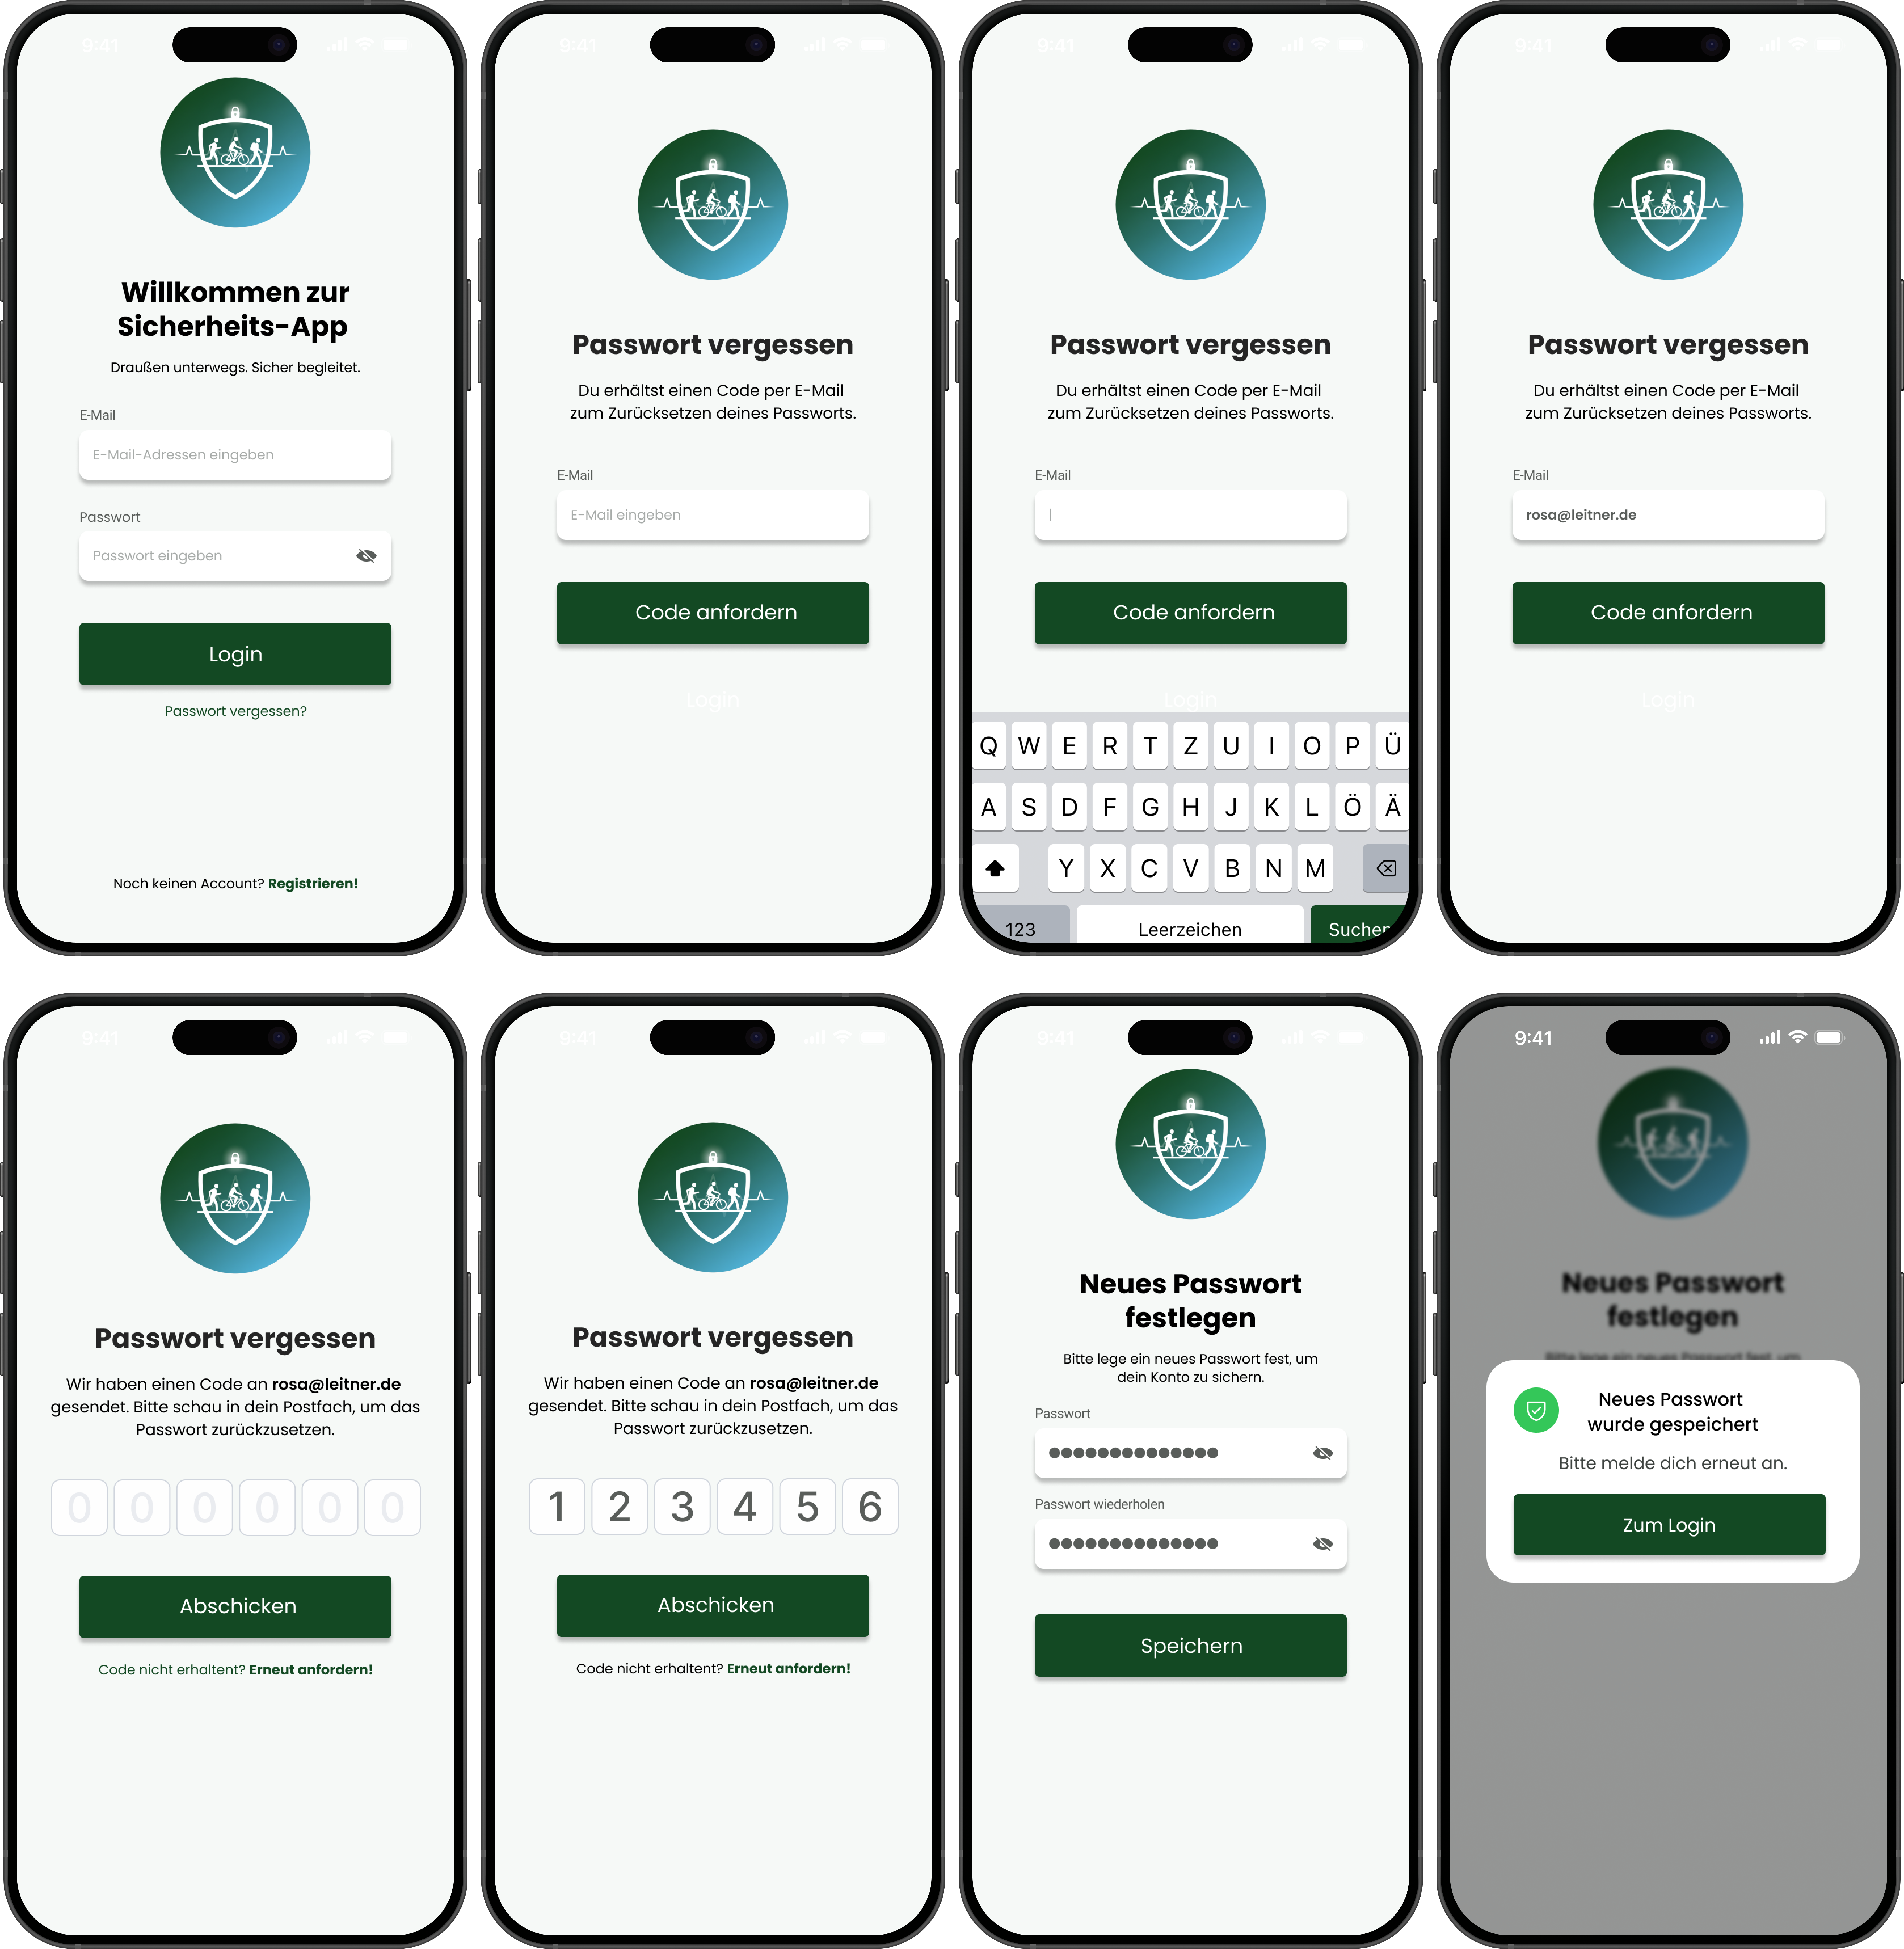
\includegraphics[width=\textwidth]{figures/login_anhang.png} 
    \caption{Prototyp: Login und Passwort vergessen(eigene Darstellung)} 
    \label{fig:login_anhang}
\end{figure}
        \chapter{Evaluation}
\label{app:evaluation}

\begin{figure}[htpb]
    \centering
    \includegraphics[width=\textwidth]{figures/Leitfaden Benutzertest_Sicherheits-App_Seite1.png}
    \caption{Leitfaden für den Benutzertest (Seite 1, eigene Darstellung)}
    \label{fig:leitfaden_test_1}
\end{figure}

\begin{figure}[htpb]
    \centering
    \includegraphics[width=\textwidth]{figures/Leitfaden Benutzertest_Sicherheits-App_Seite2.png}
    \caption{Leitfaden für den Benutzertest (Seite 2, eigene Darstellung)}
    \label{fig:leitfaden_test_2}
\end{figure}

\begin{figure}[htpb]
    \centering
    \includegraphics[width=\textwidth]{figures/UEQ_Fragebogen.png}
    \caption{UEQ-Langversion mit 26 Items \autocite{ueqonline}}
    \label{fig:ueq_fragenbogen}
\end{figure}

        % \chapter{WAVE Testergebnisse autoamtische Analyse}
\label{app:autoWAVE}
\begin{xltabular}{\linewidth}{p{2.5cm} p{2.5cm} p{4.5cm} X}
    % --- Kopfzeile (Erste Seite) ---
    \caption{WAVE Testergebnisse Startseite} \label{tab:testergebnisse-startseite-wave} \\
    \toprule
    \textbf{Prüfschritt} & \textbf{Bewertung} & \textbf{Begründung / \newline Verbesserung} & \textbf{Weitere Notizen} \\
    \midrule
    \endfirsthead

    % % --- Kopfzeile (Folgeseiten) ---
    % \caption[]{Testergebnisse Föhr: Barrierefrei} \\
    % \toprule
    % \textbf{Prüfschritt} & \textbf{Bewertung} & \textbf{Begründung / \newline Verbesserung} & \textbf{Weitere Notizen} \\
    % \midrule
    % \endhead

    % --- Fußzeilen ---
    \midrule
    \multicolumn{4}{r}{\textit{Weiter auf der nächsten Seite...}} \\
    \endfoot

    \bottomrule
    \endlastfoot

    % --- Inhalt (Sortiert) ---

    % 1. Eintrag (9.1.1 comes first)
    9.1.1.1a & 
    Teilweise erfüllt & 
    Fehlende alt-Attribute für vier Bilder & 
    Hero Image, Bild für "`Mach mal Föhr"', "`Veranstaltungen auf Föhr"' und "`Ader-Schiffe"' \\ 
    \midrule

    % 2. Eintrag (9.1.4.2 comes before 9.1.4.3)
    9.1.4.3 & 
    Teilweise erfüllt & 
    Zu geringer Kontrast, teilweise sogar nur 1,96:1, betrifft vor allem Text, der direkt auf Bildern platziert ist, insbesondere Copyright-Angaben, sowie spezifische Farbkombinationen im Layout, Z. B. die hellgrüne Textfarbe auf beigefarbenem Hintergrundenthalten. & 
    \\ 
    \midrule

    % 3. Eintrag
    9.2.4.4 & 
    Teilweise erfüllt & 
    Der Schließen-Link im Suchfeld zeigt zwar ein Icon an, hat aber keinen Namen für Screenreader (das Icon ist per aria-hidden="true" versteckt) und das title-Attribut ist nicht ausreichend \rightarrow a-Element mit aria-label="`Suchformular schließen"', um Screenreadern einen eindeutigen Linkzweck zu vermitteln. Außerdem sind die Vergrößerungs-Links in der Mediengalerie leer & 
    Suchfeld im Header Mediengalerie "`Erlebe deinen Nordseeurlaub auf der Insel Föhr"'
 \\ 
 \midrule

 % 3. Eintrag
    9.3.3.2 & 
    Teilweise erfüllt & 
    Fehlen im in zwei von drei Formularen und dort jeweils für alle Eingabefelder& 
    Quicksearch Unterkunft (Datepicker und Personenanzahl), die zweimal auf der Seite eingebunden ist
 \\ 

\end{xltabular}

\begin{xltabular}{\linewidth}{p{2.5cm} p{2.5cm} p{4.5cm} X}
    % --- Kopfzeile (Erste Seite) ---
    \caption{WAVE Testergebnisse Föhr: Barrierefrei} \label{tab:testergebnisse-barrierefrei-wave} \\
    \toprule
    \textbf{Prüfschritt} & \textbf{Bewertung} & \textbf{Begründung / \newline Verbesserung} & \textbf{Weitere Notizen} \\
    \midrule
    \endfirsthead

    % % --- Kopfzeile (Folgeseiten) ---
    % \caption[]{Testergebnisse Föhr: Barrierefrei} \\
    % \toprule
    % \textbf{Prüfschritt} & \textbf{Bewertung} & \textbf{Begründung / \newline Verbesserung} & \textbf{Weitere Notizen} \\
    % \midrule
    % \endhead

    % --- Fußzeilen ---
    \midrule
    \multicolumn{4}{r}{\textit{Weiter auf der nächsten Seite...}} \\
    \endfoot

    \bottomrule
    \endlastfoot

    % --- Inhalt (Sortiert) ---

    % 1. Eintrag (9.1.1 comes first)
    9.1.1.1a & 
    Teilweise erfüllt & 
    Fehlende alt-Attribute für ein Bild & 
    Bild "`Strandkörbe für Rollifahrer"' \\ 
    \midrule

    % 3. Eintrag
    9.2.4.6 & 
    Teilweise erfüllt & 
    Inkonsequente Überschriftenhierarchie, es wird im Artikel ein leeres h3 class="`csc-linkToTop"'>\&nbsp;</h3>-Tag als Abstandshalter verwendet und das p-Element zusätzlich zur rein visuellen Abstandserzeugung missbraucht  & 
    Im Artikel "Barrierefreies "`AQUAFÖHR"' zwischen "`Fitnessstudio"' und "`Sanitärräume"'\\ 

\end{xltabular}


\begin{xltabular}{\linewidth}{p{2.5cm} p{2.5cm} p{4.5cm} X}
    % --- Kopfzeile (Erste Seite) ---
    \caption{WAVE Testergebnisse Föhr zwischen Ebbe und Flut: Gezeitenkalender} \label{tab:testergebnisse-gezeiten-wave} \\
    \toprule
    \textbf{Prüfschritt} & \textbf{Bewertung} & \textbf{Begründung / \newline Verbesserung} & \textbf{Weitere Notizen} \\
    \midrule
    \endfirsthead

    % % --- Kopfzeile (Folgeseiten) ---
    % \caption[]{Testergebnisse Föhr: Barrierefrei} \\
    % \toprule
    % \textbf{Prüfschritt} & \textbf{Bewertung} & \textbf{Begründung / \newline Verbesserung} & \textbf{Weitere Notizen} \\
    % \midrule
    % \endhead

    % --- Fußzeilen ---
    \midrule
    \multicolumn{4}{r}{\textit{Weiter auf der nächsten Seite...}} \\
    \endfoot

    \bottomrule
    \endlastfoot

    % --- Inhalt (Sortiert) ---

    % 1. Eintrag (9.1.1 comes first)
    9.1.1.1a & 
    Teilweise erfüllt & 
    Fehlende alt-Attribute für Bilder und Videos & 
    YouTube-Video im Hero-Bereich und Bild "`FÖHRgreen"' unter "`Das könnte Sie auch interessieren…"' \\ 
    \midrule

    % 2. Eintrag (9.1.4.2 comes before 9.1.4.3)
    9.2.4.6 & 
    Teilweise erfüllt & 
    Lückenhafte Überschriftenhierarchie, Artikel beginnen mit einem p-Element und haben keine H2-Überschrift & 
    Über den einzelnen Artikeln "`Beachten Sie im Watt unbedingt folgende Hinweise:"' und  "`Das könnte Sie auch interessieren…"' \\ 
    \midrule

 % 3. Eintrag
    9.3.3.2 & 
    Teilweise erfüllt & 
    Fehlt im Formular-Eingabefeld bzw. ist leer & 
    Datepicker Gezeitenkurve
 \\ 

\end{xltabular}
        % \chapter{Lighthouse Testergebnisse autoamtische Analyse}
\label{app:autoLighthouse}
\begin{xltabular}{\linewidth}{p{2.5cm} p{2.5cm} p{4.5cm} X}
    % --- Definition Kopfzeile (Erste Seite) ---
    \caption{Lighthouse Testergebnisse Startseite} \label{tab:testergebnisse-startseite-lighthouse} \\
    \toprule
    \textbf{Prüfschritt} & \textbf{Bewertung} & \textbf{Begründung / \newline Verbesserung} & \textbf{Weitere Notizen} \\
    \midrule
    \endfirsthead

    % % --- Definition Kopfzeile (Folgeseiten) ---
    % \caption[]{Testergebnisse Startseite (Fortsetzung)} \\
    % \toprule
    % \textbf{Prüfschritt} & \textbf{Bewertung} & \textbf{Begründung / \newline Verbesserung} & \textbf{Weitere Notizen} \\
    % \midrule
    % \endhead

    % --- Fußzeilen ---
    \midrule
    \multicolumn{4}{r}{\textit{Weiter auf der nächsten Seite...}} \\
    \endfoot

    \bottomrule
    \endlastfoot

    % --- Inhalt (Sortiert) ---
    
    % 1. Eintrag (war vorher unten)
    9.1.1.1b & 
    Teilweise erfüllt & 
    Lighthouse meldet fehlende alt-Attribute bei vier Bildern. & 
    Bilder: Hero Image, "`Mach mal Föhr."', "`Veranstaltungen auf Föhr"', "`Mit den Adler-Schiffen auf Entdeckungstour"' \\ 
    \midrule


    % 2. Eintrag (war vorher oben)
    9.1.3.1a & 
    Teilweise erfüllt & 
    Die Website startet mit einer H4 (Unterkunftssuche Quicksearch). Weiterhin kommt der gleiche Container der Unterkunfssuche unten auf der Website vor unter einer H2 statt einer H3. Die semantische Reihenfolge (H1-H6) sollte immer ohne Sprünge eingehalten werden. & 
    H4: “Finde deine Unterkunft auf Föhr” \\ 
    \midrule

    % 2. Eintrag (war vorher oben)
    9.1.4.3 & 
    Teilweise erfüllt & 
    Der Mindestkontrast von 3:1 für Schriftgrößen ab 24px wird in drei Fällen nicht eingehalten & 
    Hellgrüne Texte auf beige-grauem Hintergrund Bilder: "`Ruhe. Weite. Nordsee."', "`Heute nicht auf Kosten von morgen, hier nicht auf Kosten von anderswo"', "`Kurabgabe"' \\ 

\end{xltabular}

\begin{xltabular}{\linewidth}{p{2.5cm} p{2.5cm} p{4.5cm} X}
    % --- Kopfzeile (Erste Seite) ---
    \caption{Lighthouse Testergebnisse Föhr: Barrierefrei} \label{tab:testergebnisse-barrierefrei-lighthouse} \\
    \toprule
    \textbf{Prüfschritt} & \textbf{Bewertung} & \textbf{Begründung / \newline Verbesserung} & \textbf{Weitere Notizen} \\
    \midrule
    \endfirsthead

    % % --- Kopfzeile (Folgeseiten) ---
    % \caption[]{Testergebnisse Föhr: Barrierefrei} \\
    % \toprule
    % \textbf{Prüfschritt} & \textbf{Bewertung} & \textbf{Begründung / \newline Verbesserung} & \textbf{Weitere Notizen} \\
    % \midrule
    % \endhead

    % --- Fußzeilen ---
    \midrule
    \multicolumn{4}{r}{\textit{Weiter auf der nächsten Seite...}} \\
    \endfoot

    \bottomrule
    \endlastfoot

    % --- Inhalt (Sortiert) ---

    % 1. Eintrag (9.1.1 comes first)
    9.1.1.1b & 
    Teilweise erfüllt & 
    Lighthouse meldet ein fehlendes alt-Attribut bei einem Bild. & 
    Bild: "`Strandkörbe für Rollifahrer"' \\ 
    \midrule

    % 3. Eintrag
    9.1.4.3 & 
    Teilweise erfüllt & 
    Der Mindestkontrast von 3:1 für Schriftgrößen ab 24px wird in einem Fall nicht eingehalten. & 
    Hellgrüner Text auf weißem Hintergrund "`Barrierefrei mobil mit dem cadWeazle!"'
 \\ 
    \midrule

    % 2. Eintrag (9.1.4.2 comes before 9.1.4.3)
    9.4.1.2 & 
    Teilweise erfüllt & 
    [aria-hidden=„true“]-Elemente enthalten fokussierbare untergeordnete Elemente. Das verhindert, dass dieses Element für Benutzer von assistiven Technologien wie Screenreadern verfügbar ist. & 
    Link "`Artikel weiterlesen"' im Abschnitt "`Barrierefreies AQUAFÖHR"'\\ 
\end{xltabular}

\begin{xltabular}{\linewidth}{p{2.5cm} p{2.5cm} p{4.5cm} X}
    % --- Kopfzeile (Erste Seite) ---
    \caption{Lighthouse Testergebnisse Föhr zwischen Ebbe und Flut: Gezeitenkalender} \label{tab:testergebnisse-gezeiten-lighthouse} \\
    \toprule
    \textbf{Prüfschritt} & \textbf{Bewertung} & \textbf{Begründung / \newline Verbesserung} & \textbf{Weitere Notizen} \\
    \midrule
    \endfirsthead

    % % --- Kopfzeile (Folgeseiten) ---
    % \caption[]{Testergebnisse (Detailansicht - Fortsetzung)} \\
    % \toprule
    % \textbf{Prüfschritt} & \textbf{Bewertung} & \textbf{Begründung / \newline Verbesserung} & \textbf{Weitere Notizen} \\
    % \midrule
    % \endhead

    % --- Fußzeilen ---
    \midrule
    \multicolumn{4}{r}{\textit{Weiter auf der nächsten Seite...}} \\
    \endfoot

    \bottomrule
    \endlastfoot

    % --- Inhalt (Sortiert) ---

    % 1. Eintrag (9.1.1 comes first)
    9.1.1.1b & 
    Teilweise erfüllt & 
    Lighthouse meldet ein fehlendes alt-Attribut bei einem Bild. & 
    Bild: "`FÖHRgreen"' \\ 
    \midrule

    % 2. Eintrag (9.1.4.2 comes before 9.1.4.3)
    9.1.3.1h & 
    Nicht erfüllt & 
    Formelemente benötigen ein Label. Das Label fehlt beim Datumspicker.. & 
    Datepicker unter "`Gezeitenkurve Wyk auf Föhr"' \\ 


\end{xltabular}






        % \chapter{Manuelle Überprüfung Startseite}

\begin{xltabular}{\linewidth}{p{2.5cm} p{2.5cm} p{4.5cm} X}
    % --- Definition Kopfzeile (Erste Seite) ---
    \caption{Manuelle Testergebnisse Startseite} \label{tab:testergebnisse-startseite} \\
    \toprule
    \textbf{Prüfschritt} & \textbf{Bewertung} & \textbf{Begründung / \newline Verbesserung} & \textbf{Weitere Notizen} \\
    \midrule
    \endfirsthead

    % % --- Definition Kopfzeile (Folgeseiten) ---
    % \caption[]{Testergebnisse Startseite (Fortsetzung)} \\
    % \toprule
    % \textbf{Prüfschritt} & \textbf{Bewertung} & \textbf{Begründung / \newline Verbesserung} & \textbf{Weitere Notizen} \\
    % \midrule
    % \endhead
    
    % --- Fußzeilen ---
    \midrule
    \multicolumn{4}{r}{\textit{Weiter auf der nächsten Seite...}} \\
    \endfoot

    \bottomrule
    \endlastfoot

    % --- Inhalt (Sortiert) ---
    
    % 1. Eintrag (war vorher unten)
    9.1.1.1a & 
    Teilweise erfüllt & 
    Icon Fonts haben meistens einen zugehörigen Text der die Funktion des Bedienelements beschreibt. 
In der Suche für den Abbrechen Knopf wurde das vergessen, es gibt auch kein Aria-Label oder ähnliches.
 & 
    Es wurde nicht immer das Icon selbst als aria-hidden=true markiert, wäre besser. Ist teilweise nicht möglich da Inhalt mit CSS Pseudoklasse ::after/before eingefügt wurde. \\ 
    \midrule


    % 2. Eintrag (war vorher oben)
    9.1.1.1b & 
    Nicht erfüllt & 
    Alternativtexte sind sporadisch, einige Bilder besitzen einen, viele nicht . Z.b. Hero-Image besitzt keinen alt-Text. 
Es sollte für jedes Bild entschieden werden, ob es informativ ist oder nicht und entsprechenden alt-Text hinzufügen. alt="`"' wenn nicht informativ
 & 
    \\ 
     \midrule

    % 2. Eintrag (war vorher oben)
    9.1.1.1c & 
    Vollständig erfüllt & 
    Siehe 9.1.1.1b - Es muss redaktionell entschieden werden, welche Fotografien als rein dekorativ eingestuft werden.  & 
    \\ \midrule
    
    9.1.1.1d & 
    Nicht anwendbar & 
      & 
    \\ \midrule
    
    9.1.3.1a & 
    Teilweise erfüllt & 
    Die Überschrift der Suche "`Unterkunft für deinen Nordseeurlaub finden"' ist eine H4 und überspringt somit Überschriften. Müsste oben auf der Seite H3 sein (oder H2, wenn alleinstehend). Weiter unten taucht die Suche erneut auf, auch hier H3 (oder H2)  & 
    \\ \midrule

    9.1.3.1b & 
    Nicht erfüllt & 
    Listen Markup wird genutzt für viele Objekte die keine Liste sind. z.B. einzelne Bilder wie "`Veranstaltungen auf Föhr"' oder dem Hero.  & 
    \\ \midrule

    9.1.3.1c & 
    Nicht anwendbar & 
     & 
    \\ \midrule

     9.1.3.1d & 
    Teilweise erfüllt & 
    Ein main-Element ist innerhalb eines weiteren main-Elements verschachtelt. Pro Seite darf allerdings nur ein main-Element existieren.
Das innere main-Element muss entfernt oder durch section, div oder article ersetzt werden.
 & 
    \\ \midrule

    9.1.3.1e & 
    Nicht anwendbar & 
    
 & 
    \\ \midrule

    9.1.3.1f & 
    Nicht anwendbar & 
    
 & 
    \\ \midrule

    9.1.3.1g & 
    Nicht anwendbar & 
    
 & 
    \\ \midrule

    9.1.3.1h & 
    Nicht erfüllt & 
    Label sind nicht passendem Input verknüpft. (Anreise/Abreis, Anzahl Personen)
 & 
    \\ \midrule

    9.1.3.2 & 
    Vollständig erfüllt & 
     & 
    \\ \midrule

    9.1.3.3 & 
    Vollständig erfüllt & 
     & 
    \\ \midrule

    9.1.3.4 & 
    Vollständig erfüllt & 
     & 
    \\ \midrule

    9.1.4.1 & 
    Vollständig erfüllt & 
     & 
    \\ \midrule

    9.1.4.2 & 
    Nicht anwendbar & 
     & 
    \\ \midrule

    9.1.4.3 & 
    Teilweise erfüllt & 
    Zu geringer Kontrast, teilweise sogar nur 1,96:1, betrifft vor allem Text, der direkt auf Bildern platziert ist, insbesondere Copyright-Angaben, sowie spezifische Farbkombinationen im Layout, z. B. die hellgrüne Textfarbe auf beigefarbenem Hintergrund & 
    \\ \midrule

    9.1.4.4 & 
    Vollständig erfüllt & 
     & 
    \\ \midrule

    9.1.4.5 & 
    Vollständig erfüllt & 
     & 
    \\ \midrule

    9.1.4.10 & 
    Vollständig erfüllt & 
     & 
    \\ \midrule

    9.1.4.11 & 
    Vollständig erfüllt & 
     & 
    \\ \midrule

    9.1.4.12 & 
    Vollständig erfüllt & 
     & 
    \\ \midrule

    9.1.4.13 & 
    Nicht erfüllt & 
    Tooltip bei "`merken"' verschwindet nicht bei "`esc"' Tastendruck & 
    \\ \midrule

    9.2.1.1 & 
    Vollständig erfüllt & 
     & 
    \\ \midrule

     9.2.1.2 & 
    Vollständig erfüllt & 
     & 
    \\ \midrule
    
    9.2.1.4 & 
    Vollständig erfüllt & 
     & 
    \\ \midrule

     9.2.3.1 & 
    Vollständig erfüllt & 
     & 
    \\ \midrule

     9.2.4.1 & 
    Teilweise erfüllt & 
    Überschriftenstruktur wurde bereits besprochen, ein Sprunglink zum Inhalt existiert nicht und Landmarks wie main wurden teilweise doppelt verwendet. Die drei Sachen müssen glattgezogen werden & 
    \\ \midrule

    9.2.4.2 & 
    Vollständig erfüllt & 
     & 
    \\ \midrule

    9.2.4.3 & 
    Teilweise erfüllt & 
    Tabrichtung im Header und Kontakt/Newsletter vertauscht. Wegen Flex="`row-reverse"' & 
    \\ \midrule

    9.2.4.4 & 
    Teilweise erfüllt & 
    Link-Text ist mit "`Will ich sehen"' nicht aussagekräftig, besser wäre hier "`Anreise, Prospekte, etc.w"' & 
    \\ \midrule

    9.2.4.5 & 
    Vollständig erfüllt & 
     & 
    \\ \midrule

    9.2.4.6 & 
    Vollständig erfüllt & 
     & 
    \\ \midrule

    9.2.4.7 & 
    Teilweise erfüllt & 
    Der Standard-Fokusindikator ist aufgrund der bereits vorhandenen leichten Rahmen (Kästen) der Buttons visuell nur schwer vom normalen Zustand des Elements zu unterscheide. Besser wäre die Outline Funktion mit Offset zu nutzen. 

Teilweise werden ausgeblendete Inhalte fokussiert. & 
Alle Buttons mit leichtem Rahmen
    \\ \midrule

    9.3.1.1 & 
    Vollständig erfüllt & 
     & 
    \\ \midrule

    9.3.1.2 & 
    Nicht erfüllt & 
    Wörter und Textpassagen in anderen Sprachen wurden nicht markiert, z.B. "`På dansk"', "`Newsletter"' oder "`Online-Shop"' & 
    \\ \midrule

    9.4.1.1 & 
    Teilweise erfüllt & 
    Es gibt verschachtelte main-Elemente und unzulässige Elementverschachtelung (p innerhalb span). 
Skripts wurden mit unzulässigen Modulen importiert und Verbotene Codepunkt wie U+009f wurden genutzt. 
 & 
    \\ \midrule

    9.4.1.2 & 
    Vollständig erfüllt & 
     & 
    \\ \midrule

    9.4.1.3 & 
    Nicht Anwendbar für Newsletter, da die Seite nach Anmeldung neu geladen wird & 
     & 
    \\
\end{xltabular}


        % \chapter{Manuelle Überprüfung Barrierefrei-Seite}

\begin{xltabular}{\linewidth}{p{2.5cm} p{2.5cm} p{4.5cm} X}
    % --- Definition Kopfzeile (Erste Seite) ---
    \caption{Manuelle Testergebnisse Föjr: Barrierefrei} \label{tab:testergebnisse-barrierefrei} \\
    \toprule
    \textbf{Prüfschritt} & \textbf{Bewertung} & \textbf{Begründung / \newline Verbesserung} & \textbf{Weitere Notizen} \\
    \midrule
    \endfirsthead

    % % --- Definition Kopfzeile (Folgeseiten) ---
    % \caption[]{Testergebnisse Startseite (Fortsetzung)} \\
    % \toprule
    % \textbf{Prüfschritt} & \textbf{Bewertung} & \textbf{Begründung / \newline Verbesserung} & \textbf{Weitere Notizen} \\
    % \midrule
    % \endhead
    
    % --- Fußzeilen ---
    \midrule
    \multicolumn{4}{r}{\textit{Weiter auf der nächsten Seite...}} \\
    \endfoot

    \bottomrule
    \endlastfoot

    % --- Inhalt (Sortiert) ---
    
    % 1. Eintrag (war vorher unten)
    9.1.1.1a & 
    Teilweise erfüllt & 
    Fehlendes alt-Attribut für ein Bild
 & 
    Bild "`Strandkörbe für Rollifahrer"' \\ 
    \midrule


    % 2. Eintrag (war vorher oben)
    9.1.1.1b & 
    Teilweise erfüllt & 
    alt-Texte könnten insgesamt etwas beschreibender sein, z. B. statt alt="'Friesentorte"'
alt="'Nahaufnahme einer Friesentorte mit Kaffee auf Gartentisch eines Cafés"'
oder statt alt="`Rollstuhl, Koffer oder Kinderwagen die Fähre ist barrierefrei erreichbar"'
alt="`Innenansicht Seiteneinstieg mit flacher, barrierearmer Rampe am Fähranleger in Dagebüll"'

 & Bild "`Barrierefreie Gastronomie"' und "`Barrierefreie Anreise"'
    \\ 
     \midrule

    % 2. Eintrag (war vorher oben)
    9.1.1.1c & 
    Vollständig erfüllt & 
      & 
    \\ \midrule
    
    9.1.1.1d & 
    Nicht anwendbar & 
      & 
    \\ \midrule
    
    9.1.3.1a & 
    Teilweise erfüllt & 
    Es gibt eine leere H3-Überschrift auf die eine weitere H3-Überschrift mit Text folgt. Die leere Überschrift muss entfernt werden. & 
    Barrierefreies AQUAFÖHR (zwischen Sanitärräume und Promenadenzugang)
    \\ \midrule

    9.1.3.1b & 
    Vollständig erfüllt & 
      & 
    \\ \midrule

    9.1.3.1c & 
    Nicht anwendbar & 
     & 
    \\ \midrule

     9.1.3.1d & 
    Teilweise erfüllt & 
    Ein main-Element ist innerhalb eines weiteren main-Elements verschachtelt. Pro Seite darf allerdings nur ein main-Element existieren.
Das innere main-Element muss entfernt oder durch section, div oder article ersetzt werden.
Es gibt außerdem leere p-Elemente, um vertikalen Abstand zu erzeugen.Gewünschter Abstand sollt besser über CSS gesteuert werden

 & 
    \\ \midrule

    9.1.3.1e & 
    Nicht anwendbar & 
    
 & 
    \\ \midrule

    9.1.3.1f & 
    Nicht anwendbar & 
    
 & 
    \\ \midrule

    9.1.3.1g & 
    Vollständig erfüllt & 
    
 & 
    \\ \midrule

    9.1.3.1h & 
    Vollständig erfüllt & 
 & 
    \\ \midrule

    9.1.3.2 & 
    Vollständig erfüllt & 
     & 
    \\ \midrule

    9.1.3.3 & 
    Vollständig erfüllt & 
     & 
    \\ \midrule

    9.1.3.4 & 
    Vollständig erfüllt & 
     & 
    \\ \midrule

    9.1.4.1 & 
    Vollständig erfüllt & 
     & 
    \\ \midrule

    9.1.4.2 & 
    Nicht anwendbar & 
     & 
    \\ \midrule

    9.1.4.3 & 
    Teilweise erfüllt & 
    Zu geringer Kontrast, teilweise sogar nur 1,96:1, betrifft vor allem Text, der direkt auf Bildern platziert ist, insbesondere Copyright-Angaben, sowie spezifische Farbkombinationen im Layout, z. B. die hellgrüne Textfarbe auf beigefarbenem Hintergrund & 
    \\ \midrule

    9.1.4.4 & 
    Vollständig erfüllt & 
     & 
    \\ \midrule

    9.1.4.5 & 
    Vollständig erfüllt & 
     & 
    \\ \midrule

    9.1.4.10 & 
    Vollständig erfüllt & 
     & 
    \\ \midrule

    9.1.4.11 & 
    Vollständig erfüllt & 
     & 
    \\ \midrule

    9.1.4.12 & 
    Vollständig erfüllt & 
     & 
    \\ \midrule

    9.1.4.13 & 
    Nicht erfüllt & 
    Tooltip bei "`merken"' verschwindet nicht bei "`esc"' Tastendruck & 
    \\ \midrule

    9.2.1.1 & 
    Vollständig erfüllt & 
     & 
    \\ \midrule

     9.2.1.2 & 
    Vollständig erfüllt & 
     & 
    \\ \midrule
    
    9.2.1.4 & 
    Vollständig erfüllt & 
     & 
    \\ \midrule

     9.2.3.1 & 
    Vollständig erfüllt & 
     & 
    \\ \midrule

     9.2.4.1 & 
    Teilweise erfüllt & 
    Ein main-Element ist innerhalb eines weiteren main-Elements verschachtelt. Pro Seite darf allerdings nur ein main-Element existieren.
Das innere main-Element muss entfernt oder durch section, div oder article ersetzt werden.
 & 
    \\ \midrule

    9.2.4.2 & 
    Vollständig erfüllt & 
     & 
    \\ \midrule

    9.2.4.3 & 
    Vollständig erfüllt & 
     & 
    \\ \midrule

    9.2.4.4 & 
    Teilweise erfüllt & 
    Link-Text ist mit "`Mehr erfahren"' nicht aussagekräftig, besser wäre hier "`Infos zur barrierefreien Anreise"' & Artikel "`Barrierefreie Anreise
    \\ \midrule

    9.2.4.5 & 
    Nicht erfüllt & 
    Unterseite ist nur über das Suchfeld auffindbar und z. B. nicht auf der Seite "`Barrierefreie Anreise"' verlinkt & 
    \\ \midrule

    9.2.4.6 & 
    Vollständig erfüllt & 
     & 
    \\ \midrule

    9.2.4.7 & 
    Teilweise erfüllt & 
    Der Standard-Fokusindikator ist aufgrund der bereits vorhandenen leichten Rahmen (Kästen) der Buttons visuell nur schwer vom normalen Zustand des Elements zu unterscheide. Besser wäre eine zusätzliche, kontrastreiche farbliche Hervorhebung (z. B. einen dicken, farbigen Rahmen oder eine Hintergrundfarbänderung)& 
    Alle Buttons mit leichtem Rahmen
    \\ \midrule

    9.3.1.1 & 
    Vollständig erfüllt & 
     & 
    \\ \midrule

    9.3.1.2 & 
    Nicht anwendbar & 
    & 
    \\ \midrule

    9.4.1.1 & 
    Teilweise erfüllt & 
    Es gibt verschachtelte main-Elemente, leere id-Attribute, doppelte id-Werte, ungültige Attributwerte (required) sowie unzulässige Elementverschachtelung (p innerhalb span). 

Zweites main-Element entfernen, gültige, eindeutige IDs sowie required="required" verwenden, p entweder direkt verwenden oder muss oder n ein div-Element einbetten. 
 & 
    \\ \midrule

    9.4.1.2 & 
    Vollständig erfüllt & 
     & 
    \\ \midrule

    9.4.1.3 & 
    Vollständig erfüllt & 
     & 
    \\
\end{xltabular}


        % \chapter{Manuelle Überprüfung Gezeiten-Seite}

\begin{xltabular}{\linewidth}{p{2.5cm} p{2.5cm} p{4.5cm} X}
    % --- Definition Kopfzeile (Erste Seite) ---
    \caption{Manuelle Testergebnisse Föhr zwischen Ebbe und Flut: Gezeitenkalender} \label{tab:testergebnisse-gezeiten} \\
    \toprule
    \textbf{Prüfschritt} & \textbf{Bewertung} & \textbf{Begründung / \newline Verbesserung} & \textbf{Weitere Notizen} \\
    \midrule
    \endfirsthead

    % % --- Definition Kopfzeile (Folgeseiten) ---
    % \caption[]{Testergebnisse Startseite (Fortsetzung)} \\
    % \toprule
    % \textbf{Prüfschritt} & \textbf{Bewertung} & \textbf{Begründung / \newline Verbesserung} & \textbf{Weitere Notizen} \\
    % \midrule
    % \endhead
    
    % --- Fußzeilen ---
    \midrule
    \multicolumn{4}{r}{\textit{Weiter auf der nächsten Seite...}} \\
    \endfoot

    \bottomrule
    \endlastfoot

    % --- Inhalt (Sortiert) ---
    
    % 1. Eintrag (war vorher unten)
    9.1.1.1a & 
    Teilweise erfüllt & 
    Links mit href="`javascript:void(0)"' für "`Artikel weiterlesen/weniger anzeigen"' haben aria-hidden="`true"' - diese sollten echte Buttons sein. Der Submit-Button der Suche hat nur title="`Suche abschicken"', aber keinen sichtbaren Text. Besser wäre ein aria-label. Der "`merken"'-Button hat keinen ausreichend beschreibenden Text für Screenreader.
 & 
    Bild "`Strandkörbe für Rollifahrer"' \\ 
    \midrule


    % 2. Eintrag (war vorher oben)
    9.1.1.1b & 
    Teilweise erfüllt & 
    Lighthouse meldet ein fehlendes alt-Attribut bei einem Bild.
 & Bild: "`FÖHRgreen"'
    \\ 
     \midrule

    % 2. Eintrag (war vorher oben)
    9.1.1.1c & 
    Vollständig erfüllt & 
      & 
    \\ \midrule
    
    9.1.1.1d & 
    Nicht anwendbar & 
      & 
    \\ \midrule
    
    9.1.3.1a & 
    Vollständig erfüllt & 
    Überschriften sind vorhanden und strukturiert (H1: "`Gezeiten"', H2/H3: Unterüberschriften). Die Hierarchie erscheint logisch. & 
    \\ \midrule

    9.1.3.1b & 
    Vollständig erfüllt & 
      & 
    \\ \midrule

    9.1.3.1c & 
    Nicht anwendbar & 
     & 
    \\ \midrule

     9.1.3.1d & 
    Vollständig erfüllt & 
    Der Inhalt ist in logische Abschnitte gegliedert (Gezeiteninfo, Sicherheitshinweise, Wassertemperatur, Wetter)

 & Gute visuelle und semantische Gliederung erkennbar.
    \\ \midrule

    9.1.3.1e & 
    Nicht anwendbar & 
    
 & 
    \\ \midrule

    9.1.3.1f & 
    Nicht anwendbar & 
    
 & 
    \\ \midrule

    9.1.3.1g & 
    Vollständig erfüllt & 
    
 & 
    \\ \midrule

    9.1.3.1h & 
    Nicht erfüllt &  
    Formelemente benötigen ein Label. Das Label fehlt beim Datumspicker. Datepicker unter "`Gezeitenkurve Wyk auf Föhr"' &
    Mit dem Jahreswechsel hat sich die Webseite geändert. Es gibt keine Gezeitenkurve mehr, sondern stattdessen ein downloadbares PDF. Die Analyse fand davor statt.
    \\ \midrule

    9.1.3.2 & 
    Vollständig erfüllt & 
    Die Inhaltsreihenfolge ist logisch: Navigation, Hauptinhalt, Zusatzinformationen, Footer. & 
    Die Lesereihenfolge entspricht der visuellen Reihenfolge.
    \\ \midrule

    9.1.3.3 & 
    Vollständig erfüllt & 
    Keine rein visuellen Anweisungen werden auf der Webseite verwendet. & 
    Inhalte sind auch ohne Farb- oder Positionsinformationen verständlich.
    \\ \midrule

    9.1.3.4 & 
    Vollständig erfüllt & 
     & 
    \\ \midrule

    9.1.4.1 & 
    Vollständig erfüllt & 
     & 
    \\ \midrule

    9.1.4.2 & 
    Nicht anwendbar & 
     & 
    \\ \midrule

    9.1.4.3 & 
    Teilweise erfüllt & 
    Im Header hat die weiße Schrift auf dem Video-Hintergrund einen Kontrast von 1.1 und damit gering. &
    Auf manchen Bildern unter "`Das könnte Sie auch interessieren…"' ist die Schrift des Copyrights Teil des Fotos und nicht als Schrift zu inspektieren. Man kann annehmen, dass hier der Kontrast nicht ausreichend wäre. 
    \\ \midrule

    9.1.4.4 & 
    Vollständig erfüllt & 
     & 
    \\ \midrule

    9.1.4.5 & 
    Vollständig erfüllt & 
     & 
    \\ \midrule

    9.1.4.10 & 
    Vollständig erfüllt & 
     & 
    \\ \midrule

    9.1.4.11 & 
    Vollständig erfüllt & 
     & 
    \\ \midrule

    9.1.4.12 & 
    Vollständig erfüllt & 
     & 
    \\ \midrule

    9.1.4.13 & 
    Vollständig erfüllt & 
     & 
    \\ \midrule

    9.2.1.1 & 
    Vollständig erfüllt & 
     & 
    \\ \midrule

     9.2.1.2 & 
    Vollständig erfüllt & 
     & 
    \\ \midrule
    
    9.2.1.4 & 
    Vollständig erfüllt & 
    Keine benutzerdefinierten Tastatur-Kurzbefehle erkennbar. & 
    \\ \midrule

     9.2.3.1 & 
    Vollständig erfüllt & 
    Keine automatisch animierten oder flackernden Inhalte erkennbar.     & 
    \\ \midrule

     9.2.4.1 & 
    Nicht anwendbar & 
    Es sind keine Sprunglinks vorhanden.& 
    \\ \midrule

    9.2.4.2 & 
    Vollständig erfüllt & 
    Seitentitel ist aussagekräftig: "Föhr zwischen Ebbe und Flut: Gezeitenkalender" & 
    \\ \midrule

    9.2.4.3 & 
    Vollständig erfüllt & 
     & 
    \\ \midrule

    9.2.4.4 & 
    Teilweise erfüllt & 
    Unter "`Das könnte Sie auch interessieren…"', haben die verlinkten Seiten alle den Text "`will ich sehen"'. Hier könnte etwas aussagekräftiges gewählt werden. Zum Beispiel "`Mehr erfahren"' für den Link zum Schlafstrandkorb. &
    \\ \midrule

    9.2.4.5 & 
    Vollständig erfüllt & 
    Mehrere Navigationswege vorhanden: Hauptmenü, Footer-Links, Breadcrumbs (zurück zur Startseite). & 
    \\ \midrule

    9.2.4.6 & 
    Vollständig erfüllt & 
     & 
    \\ \midrule

    9.2.4.7 & 
    Vollständig erfüllt & 
    Standard-Browser-Fokusring ist meistens sichtbar.& 
    \\ \midrule

    9.3.1.1 & 
    Vollständig erfüllt & 
    Die Seite ist auf Deutsch und hat lang="`de"' im HTML-Tag. & 
    \\ \midrule

    9.3.1.2 & 
    Nicht anwendbar & 
    &  Im Menü gibt es den Link "`På dansk"', der selbsterklärend ist und zu einer Seite mit Informationen zu Föhr auf Dänisch weiterleitet.
    \\ \midrule

    9.4.1.1 & 
    Teilweise erfüllt & 
    Blockquote wird falsch verwendet. & 
    \\ \midrule

    9.4.1.2 & 
    Vollständig erfüllt & 
     & 
    \\ \midrule

    9.4.1.3 & 
    Nicht Anwendbar für Newsletter, da die Seite nach Anmeldung neu geladen wird & 
     & 
    \\
\end{xltabular}


        %\input{appendices/appendix2}
        
        % add lists of figures, tables and listings to the appendix
        \listoffigures
        \listoftables
        %\lstlistoflistings
        
        % add acronyms
        %\printglossary[type=\acronymtype, title=Abkürzungsverzeichnis, toctitle=Abkürzungsverzeichnis, numberedsection] 
        

    \end{appendix}
    %\newpage
    %\input{appendices/erklaerung}

    %%%%%%%%%%%%%%%%%%%%%%%%%%%%%%%%
    %%%%%%%%%%%%%%%%%%%%%%%%%%%%%%%% 
    
\end{document}
